\documentclass[a4paper,11pt]{report}
\usepackage[left=3.5cm, right=2cm, top=2cm, bottom=2cm]{geometry}
\usepackage{fancyhdr}
\usepackage[nottoc,notlof,notlot]{tocbibind}
\usepackage{graphicx}
\usepackage{float}
\usepackage{tocloft}
\usepackage{setspace}
\usepackage{natbib}
\usepackage{chngcntr}
\usepackage{titlesec}
\usepackage{comment}
\usepackage{booktabs}
\usepackage{amsmath}
\usepackage{csvsimple}
\usepackage{booktabs}
\usepackage{xcolor}
\usepackage{hyperref}
\usepackage{subcaption}
\usepackage{siunitx}
\usepackage{comment}
\usepackage{ragged2e}
\usepackage{array}
\usepackage{multirow}
\usepackage{natbib}
\usepackage{wrapfig}


\newcommand{\dk}[1]{\textbf{\color{red}#1}}
\newcommand{\qs}[1]{\textbf{\color{blue}#1}}

\title{Title of the Capstone Project}
\date{}

\titleformat{\chapter}[block]{\normalfont\Large\bfseries}{\thechapter.}{1em}{}
\titlespacing*{\chapter}{0pt}{\baselineskip}{\baselineskip}
\pagestyle{fancy}
\fancyhf{}
\fancyfoot[C]{\thepage}
\renewcommand{\headrulewidth}{0pt}
\renewcommand{\footrulewidth}{0pt}
\counterwithout{figure}{chapter}
\counterwithout{table}{chapter}

\setcounter{tocdepth}{4}
\setcounter{secnumdepth}{4}

\begin{document}

\begin{titlepage}
    \newcommand{\HRule}{\rule{\linewidth}{0.5mm}}
    \centering
    \vspace*{1.8cm}
    
    \textbf{\Large Department of Statistics 2022/2023}\\
    \vspace{0.8cm}
    
    \HRule\\[0.8cm]
    
    {\LARGE \bfseries Using Remote Sensing to Improve Efficiency of Water Pollution Monitoring}\\[0.4cm] 
    
    \HRule\\[1.5cm]
    
    \vspace{0.8cm}
    
    \textbf{Candidate Numbers:}\\
    52208\\44384\\44326

    \vfill
    
    \textbf{Submitted for the Master of Science,}\\
    \textbf{London School of Economics, University of London}\\
    \vspace{1.8cm}
    
\end{titlepage}

\pagenumbering{roman}
\tableofcontents



\newpage


\listoffigures
\listoftables


\chapter*{Executive Summary}

\addcontentsline{toc}{chapter}{Executive Summary}
\onehalfspacing
\begin{comment}
\qs{Description of requirement: 
Executive summary: a summary of the work in no more than 1500 words (not more than 3
pages). This is an integral component of the Capstone report. The executive summary should
provide a succinct and at the same time thorough overview of the main findings and
recommendations. It should enable the reader to become acquainted with the content of
the capstone report without having to read it all.}
\end{comment}

This research project aims to investigate how predictive models can be built to make predictions about sewage pollution from ocean satellite data along the United Kingdom shoreline. The possibilities for using satellite images to monitor water quality was highlighted by a whitepaper published under EOMORES (Earth Observation-based Services for Monitoring and Reporting of Ecological Status), which is funded by an EU research and innovation programme \citep{papathanasopoulou2019satellite}. 

Monitoring sewage pollution with satellite data can significantly reduce costs while also improving the scope of sewage pollution monitoring spatially compared to current monitoring methods. Current methods of measurement, including event duration monitors or manual observation, are effective only to a fairly local scope, in addition to being very costly. 

Satellite data was extracted from the Copernicus Marine Store, which is managed under the European Union's Earth Observation Programme. Two datasets from two different satellites were extracted, and both provided data on key ocean physical variables relevant to sewage pollution were extracted. One dataset (S2) provides higher spatial resolution data at a lower temporal frequency, and the other (S3) provides the opposite. The sewage pollution labelled dataset was taken from the Environment Agency. 

Exploration data analysis was performed on the datasets, informing our decision to engineer features from raw satellite data and to compare various binary classifiers across various settings as our main methodology. A comparison across Sentinel-2 and Sentinel-3 data led to the decision to proceed primarily with S3 data for our primary analyses and evaluations. We found that there was a significant amount of missing data across both spatial and temporal dimensions, which informed our decision to fill missing data in a twofold manner: first across spatial gaps with mean values, then across temporal gaps with either 0 or -10. 

Upon closer examination of the features, there was increasing variability as grid size grew, with specific features like BBP, CDM, KD490, and CHL decreasing in offshore waters. Pearson's correlation indicated that features such as SPM have a higher potential in predicting pollution risk. The association of high values of BBP and SPM with increased pollution risks highlighted the relationships between CHL, KD490, and ZSD. However, the linear correlations may not fully capture the intricate relationships, suggesting that machine learning could offer deeper insights.


The four key supervised learning model classes that were explored are logistic regression, random forest, multi-layer perception and convolutional neural network. These four models were chosen to enable comparison across a wide range of models that take in different input data. Logistic regression, random forest and multi-layer perception were trained and tested on engineered features datasets based on the hypothesis that they would benefit from some form of aggregation. The convolutional neural network models were trained and tested on the raw input data by treating the input data as an image, treating features as channels and stacking the features for each spatial window. A baseline model was also constructed to compare the performance of the four key model classes which made random predictions based on the proportion of positive samples in our dataset. Imbalanced data was a key challenge for the project, which was addressed through classifier construction and various hyperparameter tuning methods, such as introducing oversampling and weighted binary classification losses for neural network models. 

Through cross-comparisons and evaluations, our analysis found that Random Forest emerged as the most proficient classifier, particularly using data extract for each bathing water size with a 5.1km × 5.1km window size from the engineered features dataset from Sentinel-2 data. Performance trends differed based on several factors, including temporal categories like year and month, regions, and weather data was engineered. While some models excelled with raw data, others, such as Random Forest and Logistic Regression, particularly benefited from feature engineering. Data with higher spatial resolution typically led to better model outcomes. However, the complexities introduced by capturing data with a larger geographical area didn't consistently yield superior results. Despite our diligent efforts, the classifiers' performance remained relatively low, reflecting the challenges and complexities in predicting sewage pollution from satellite data. 

The paper concludes by highlighting several limitations of the project and proposes directions for further investigation and research. These include suggestions for increasing data size and for creating more complex and sophisticated models, such as by incorporating lagged historical data, and confounding signals such as weather reports, bathymetry data, etc. 


\chapter{Introduction}
\pagenumbering{arabic}
\onehalfspacing
Sewage pollution presents a significant ecological challenge in the UK. According to data released by the Environment Agency earlier this year \citep{ea}, the number of sewage spills in 2022 reached a total of 301,091 incidents, averaging 824 spills per day. Water companies across England have become overly reliant on using storm overflows to dump raw sewage into our waters rather than investing in infrastructure improvements. This raw sewage contains a mixture of bacteria, viruses, harmful chemicals, and microplastics - a recipe for disaster for our oceans.

Current methods of measurement, such as event duration monitors (EDMs) or manual observation, have notable limitations when it comes to monitoring sewage pollution. The former is not only expensive but its effectiveness is limited to the locations where the equipment is installed. The latter method, while somewhat more versatile, still suffers from constraints in both temporal and spatial scope, as it requires human observers to conduct the measurements.

Considering these challenges, the use of satellite images for water pollution monitoring has been proposed as a potential solution. Theoretically, satellite imaging offers many advantages over traditional methods, including lower costs, broader coverage, greater scalability, and the potential for more timely warnings. The potential for using satellite images to monitor water quality has been highlighted by a whitepaper published under EOMORES (Earth Observation-based Services for Monitoring and Reporting of Ecological Status), which is funded by an EU research and innovation programme \citep*{papathanasopoulou2019satellite}.

In order to complement existing methods for monitoring sewage pollution spills in the UK, in this project, we aim to use satellite remote-sensing datasets, which provide satellite images with temporal and spatial information about water bodies, along with past water pollution monitoring data, to model and predict sewage pollution in the UK. Remote sensing satellite data was taken from the Copernicus Marine Services, and we took data with variables relevant to sewage pollution across two different satellites for comparison and contract. Data from satellite Sentinel-2 has a higher spatial resolution but lower temporal frequency, while data from Sentinel-3 has a lower spatial resolution but higher temporal frequency.

Our findings revealed that the Random Forest model, which utilized engineered features from the Sentinel-2 dataset within a 5.1km x 5.1km window, outperformed other classifiers. The model's effectiveness varied based on factors such as year, month, and region. Although predictive capacity decreased yearly, it rose monthly during the bathing season we investigated (May-September). The east coast of England emerged as a particularly challenging region for predictions. Notably, our results highlighted the significant impact of feature engineering. Traditional algorithms benefited more from these engineered features, and superior results were achieved using higher-resolution Sentinel-2 data. However, expanding the search areas around each data extraction site did not show a consistent trend in performance improvement. A major challenge we faced was the high incidence of False Positive Rate in many of our models; in other words, a significant number of cases with normal pollution risk were incorrectly identified as having increased pollution risk. Nevertheless, despite these constraints, our study provides foundational insights that can enhance model performance, setting the stage for future research endeavours.

The remainder of the report is structured as follows. First, a more detailed problem formulation is presented, introducing the datasets used. This is followed by exploratory data analysis and preliminary data preprocessing on the dataset. Predictive models for the problem are then presented. Finally, there are the final results of our datasets with the selected models. 

\chapter{Datasets}
This section introduces datasets utilised and presents exploratory data analysis on the data, which was performed to inform data pre-processing steps and refine our methodology. It was decided that the scope of the project would be from 2020 to 2022, taking three years of data balances between having a manageable dataset size and also having sufficient data to perform our analyses. 

We first explored the bathing water quality data provided by the Environment Agency, which gives us true labels for sewage pollution, and satellite data, from which we hope to build models and make predictions on sewage pollution. As the spatial nature of the satellite data made it difficult to perform analyses directly on the data, we engineered features from the satellite data and performed analyses on the engineered feature data combined with true labels for sewage pollution to better understand correlations and patterns within the satellite data with regards to sewage pollution. 

\section{Bathing Water Data}

\subsection{Dataset Overview}

The bathing water quality dataset is open data collected by the Environment Agency, which reflects the water quality of bathing sites along the coast and inland to ensure the water is safe and clean for swimming and other water activities. The Environment Agency is a public authority sponsored by the United Kingdom government's Department for Environment, Food \& Rural Affairs (DEFRA) with the responsibility for environmental conservation in England.

The datasets were sourced directly from the official website of the Environmental Agency
\footnote{\href{https://environment.data.gov.uk/bwq/profiles/data.html}{https://environment.data.gov.uk/bwq/profiles/data.html}}. For the purpose of this project, the focus was narrowed down to England, and the timeline was set starting from January 2020. The selections made were 'Bathing Water Site Details' and 'History of Pollution Risk Forecasts,' resulting in two CSV files. The two datasets were utilized to obtain a comprehensive understanding of historical water quality:

\begin{enumerate}
\item \textbf{Bathing water site details} dataset contains data on 430 bathing water sites in England that have been assessed by the Environment Agency. This dataset includes details such as the site ID, site name, coordinates, the district to which each site belongs, and the years the sites were designated.

\item \textbf{History of pollution risk forecasts} dataset provides daily information about warning notices and risk levels for each site. Here, the 'warning' feature offers a categorical textual representation of any abnormalities or anomalies observed, while the 'riskLevelLabel' feature holds binary values: 'normal' or 'increased,' indicating whether a higher observed risk is present or not. As per the Environmental Agency's website, “Pollution risk forecasts” are essentially predictions formulated by factors like rainfall to assess potential risks of diminished bathing water quality. It is crucial to highlight that such forecasts are not available for all bathing waters. Some bathing sites, unaffected by issues like rainfall-induced pollution, might lack these predictive data points. Consequently, there's a possibility of skewed or incomplete assessments of water risk.

\end{enumerate}

\subsection{Data Wrangling}

\subsubsection{Dataset \#1: Bathing water site details}
From the dataset, only relevant columns such as the site ID, the district, and the coordinates (longitude and latitude) of each site were retained. To enable a future comparison of model performance across various regions, a new column named “region” was introduced using the existing district information. This column encompasses eight distinct areas: the North East, North West, Yorkshire and The Humber, East Midlands, West Midlands, South East, East of England, and South West. The dataset was subsequently saved as \verb|pollution_risk_forecasting.csv|.

\subsubsection{Dataset \#2: History of pollution risk forecasts}

The column 'Warning' was deemed redundant since the risk level labels already capture the essential state of risk of the bathing water, and the descriptions within the warning column were not seen as adding significant value to the pollution prediction task. In terms of data representation, a binary variable y = $\{0, 1\}$ was used to indicate `normal` and `increased` for the `riskLevelLabel` column instead of the character data type for ease of analysis and computational efficiency.

The timestamps for each risk forecast were simplified to the year-month-date format, eliminating the specific times of prediction and publication since most of the predictions for each site are updated on a daily basis. For dates that had multiple records, only one was retained. If any record for a particular day pointed to an increased risk, the day was labelled as `increased`; otherwise, it was categorized as `normal`. The final, refined dataset was stored as \verb|site.csv|.

\subsection{Imbalanced Data} 

In the historical dataset of pollution risk forecasts, due to the small number of entries in each warning category, no clear differences between groups could be observed. Also, the feature warning merely provides detailed explanations of the risk level labels, which effectively summarize the warnings. Therefore, we continue with only the feature risk level label without considering the feature warning in our analysis.

The dataset presented a significant imbalance in the distribution of water risk level labels, as shown in figure \ref{fig:label}. A majority of the records were classified as 'normal,' with only a small number of records categorized as having an 'increased' risk level label. In the pollution risk forecasts dataset, which contains risk level labels for each site from 2020 to 2022, no more than 3\% of the records are labelled with an 'increased' risk level.


\begin{figure}
\centering
    \includegraphics[width=0.5\textwidth]{images/riskLevelLabel.png}
    \caption{Distribution of 'riskLevelLabel'} 
    \label{fig:label}
\end{figure}


\subsection{Visualising Missing Values}

According to the official website of the Environmental Agency \citep{Bathing}, the bathing water season in England runs from 15 May to 30 September. This period attracts the highest number of visitors to the bathing waters, so water quality is consistently monitored during this time frame. As a result, the risk forecasting dataset in this study primarily encompasses daily pollution risk forecasts from this season.

Figure \ref{fig:bath2} illustrates the count of sites with pollution risk forecasting records via a calendar plot. In this visual representation, each square denotes a day; individual subplots correspond to each year, with the y-axis representing the day of the week and the x-axis indicating the month. Darker shades signify dates when a higher number of sites reported data, while lighter shades or white represent fewer sites or potentially none.

It's worth highlighting that not all 430 sites provided risk forecasting data throughout the three years. Specifically, 421 sites contributed data in both 2020 and 2022, whereas 2021 saw input from only 419 sites. Moreover, certain dates, like 20 August and 3 September 2020, lack records for most sites.

\begin{figure}[H]
\centering
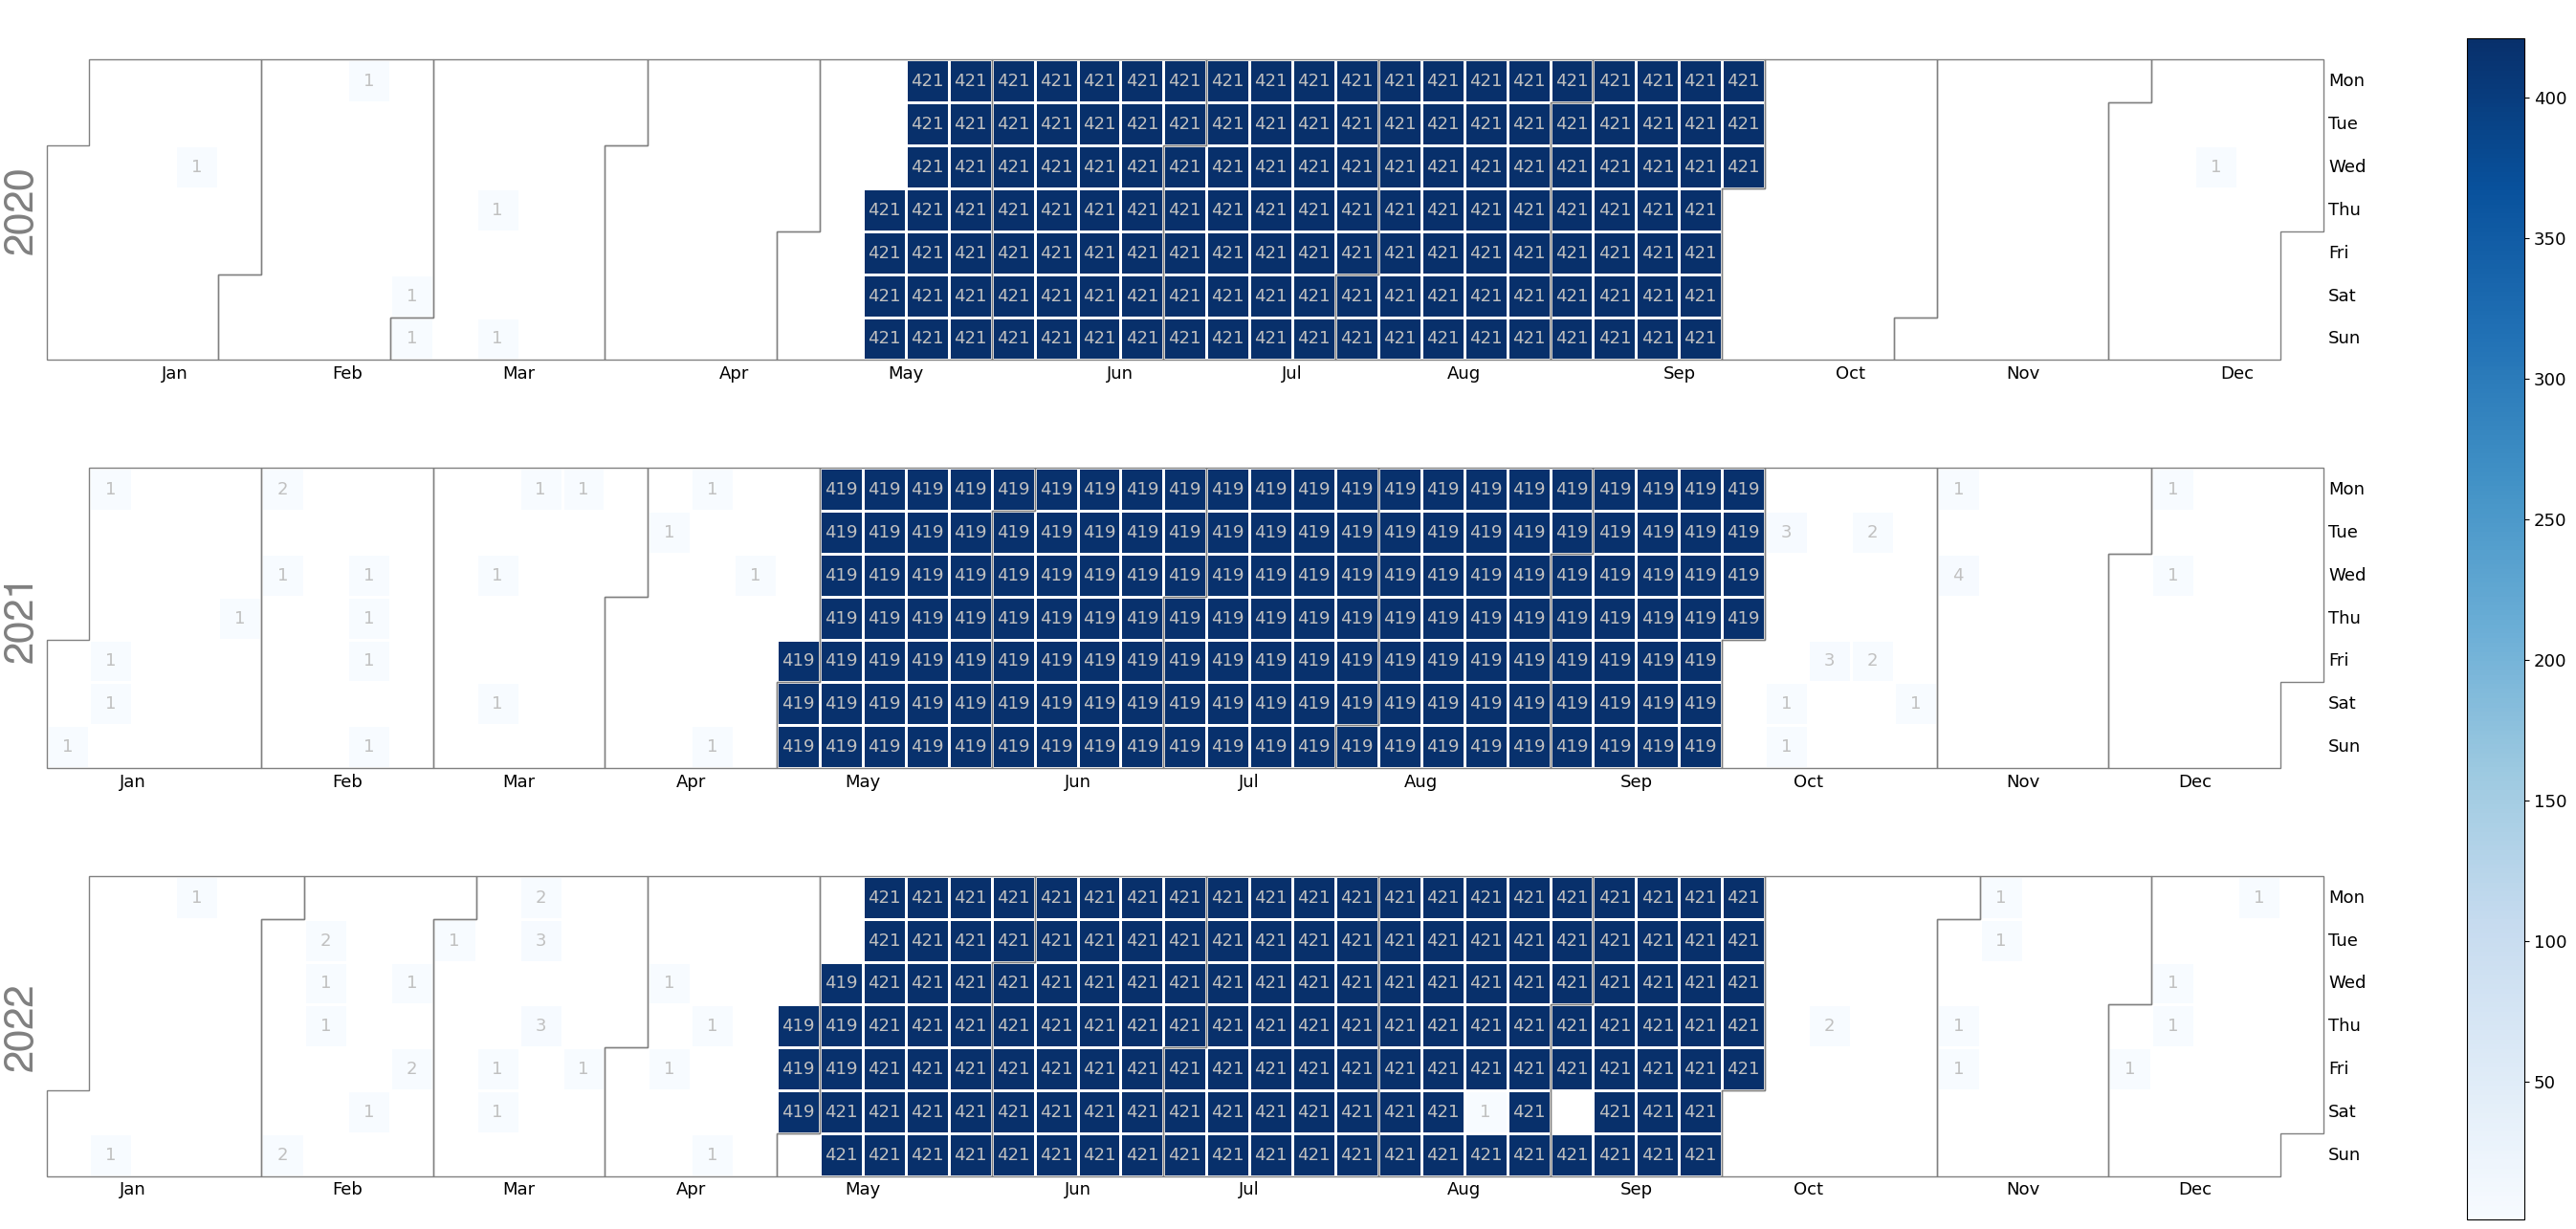
\includegraphics[width=\textwidth]{images/Bathing_water_missing_data.png}
\caption{Daily Count of Sites Reporting Pollution Risk Forecasts (2020-2022)}
\label{fig:bath2}
\end{figure}

\section{Satellite Data}
\subsection{Dataset Overview}
Satellite data were taken from the Copernicus Marine Service \footnote{https://marine.copernicus.eu/}, which provides free and open marine data and services. Copernicus is part of the European Union's Space programme which focuses on Earth observation. 

Two suitable datasets were preliminarily found with data that seems relevant to sewage pollution. The major difference between the two datasets was that one was taken from the Sentinel-2 Earth observation mission (S2), which provides higher spatial resolution data at a lower temporal frequency, while the other was taken from the Sentinel-3 Earth observation mission (S3), which provides lower spatial resolution data but at a higher temporal frequency. Both datasets were extracted for further examination, and the details of these datasets are presented below.

\subsubsection{Sentinel 2 Data}
\label{sec:Sentinel2}

Titled 'North West Shelf Region, Bio-Geo-Chemical, L4, interpolated daily observation' \footnote{\href{https://data.marine.copernicus.eu/product/OCEANCOLOUR_NWS_BGC_HR_L4_NRT_009_209/description}{https://data.marine.copernicus.eu/product/OCEANCOLOUR\_NWS\_BGC\_HR\_L4\_NRT\_009\_209/description}}, the dataset taken from S2 gives data along a 20km coastal zone around the North West Shelf Region, which includes the entire United Kingdom, at a spatial resolution of 0.1 km x 0.1km. 

For each point, data is available for three variables: mass concentration of chlorophyll-a in seawater (CHL), mass concentration of suspended matter in seawater (SPM), and seawater turbidity (TUR). The EOMORES white paper has suggested that an increase in sewage pollution is correlated with an increase in CHL, SPM and TUR values \citep{papathanasopoulou2019satellite}. CHL concentration is a potential proxy for phytoplankton abundance and intensity, while TUR and SPM reveal information about the transparency of the seawater. 

The dataset has a processing level of 'L4' and contains daily averages for the three features. Raw optical imagery was first gathered by S2 satellites and then goes through several layers of pre-processing. L4 indicates on top of standard pre-processing, interpolation, and gap-filling were also done on cloudy areas and when there was no overpass on certain days with algorithmic approaches. The higher level of pre-processing is especially pertinent here as S2 satellites typically have a 10-day revisit cycle. Note that however, interpolation is not always possible if there are too many clouds. By working with a dataset with a higher level of pre-processing, the dataset is increased despite the lower frequency data and hopefully gives us more signals to work with. 

\subsubsection{Sentinel 3 Data}

Titled 'North Atlantic Ocean Colour Plankton, Reflectance, Transparency and Optics MY L3 daily observations'\footnote{\href{https://data.marine.copernicus.eu/product/OCEANCOLOUR_ATL_BGC_L3_MY_009_113/services}{https://data.marine.copernicus.eu/product/OCEANCOLOUR\_ATL\_BGC\_L3\_MY\_009\_113/services}}, this dataset taken from S3 gives data on the North Atlantic Ocean, which surrounds the entire United Kingdom, at a spatial resolution of 1 km x 1 km. 

For each point, data is available for 6 variables: Chlorophyll-a (CHL), Suspended Matter (SPM), Secchi Transparency Depth (ZSD), Diffuse Attenuation (KD490), Particulate Backscattering (BBP), and Absorption Coefficient (CDM). All of these variables are either plankton, reflectance, transparency, or optics measures. They have also been suggested to be important for water pollution by the EOMORES whitepaper \citep{papathanasopoulou2019satellite}, as ZSD, KD490, BBP and CDM all give additional information regarding water transparency. 

The dataset has a processing level of 'L3' and contains daily averages for the three features. 'L3' indicates it has a lower standard of pre-processing than 'L4' and thus the S2 dataset. S3 has a revisit time of under two days, which is much higher than that of S2 data.


\subsection{Data Extraction}

The Copernicus Marine Service has established methods of data access that allow data to be downloaded programmatically. The process described below was used to download both our S2 and S3 datasets. 

For each dataset, data is available on the points on a fixed grid that stretches over the region covered, with the space between the points approximately defined by the spatial resolution of the dataset. This grid remains consistent over time. Thus, for each time-site pair, every site was first 'snapped' onto the grid of data points for our chosen Copernicus dataset based on its true latitude and longitude, such that the point closest to the site's true location on the grid acts as a proxy for the site. Then, data points were taken in a square with the site-proxy at the centre. Taking a square with dimension $d$ is referred to as taking a $d \times d$ window.

The MOTU Service is an advanced web server designed to manage and extract extensive oceanographic datasets\footnote{\href{https://help.marine.copernicus.eu/en/articles/4796533-what-are-the-motu-apis}{https://help.marine.copernicus.eu/en/articles/4796533-what-are-the-motu-apis}} which enables users to minimize data volume, select specific data parameters, and obtain detailed dataset information while ensuring the security of their login credentials. 

For this study, data was retrieved using the MOTU Client API. The approach involved looping through various sites and making an API call for each one. Looping through each site for the download reduces the downloaded file size as each call must encompass a square area, defined by the leftmost and rightmost longitude and the topmost and bottommost latitude. Other specifications for the API call include providing a time frame (1 January 2020 to 31 December 2022) and variables of interest, which were defined according to the dataset being downloaded. Service ID, product ID, website credentials, output filename, and directories were inputted accordingly. A maximum of one datapoint can be obtained each day. After obtaining 430 .nc files through this process, they were combined into one large comma-separated-value (CSV) file, where each row of the file contains the values of the relevant variables for a specific time, site and coordinate. 

\subsection{Comparison Between S2 and S3 Data}
Preliminarily, data was extracted for a $51 \times 51$ window for S2 data (covering an area of approximately 5.1km $\times$ 5.1km) and for a $15 \times 15$ window for S3 data (covering an area of approximately 15km $\times$ 15km). A $51 \times 51$ window was taken for S2 as although it was hoped that a larger dataset could be used to match the area covered by S3, the dataset became too difficult to download and manage. On the other hand, reducing the window size of S3 may lead to problems with using a neural network for our models. Note that this means that the data extracted for S2 covers an area of approximately \SI{225}{\km\squared}, which is 8.65 times the approximately \SI{26}{\km\squared} covered by S3. 

Table \ref{tab:s2_s3_comparison} presents a preliminary comparison between the data we get for S2 and S3 for the above window sizes. Note that null values are an issue for both S2 and S3 data. Though S3 has a revisit cycle of 1-2 days, data is completely absent on cloudy days. The 10-day revisit cycle for S2 also means that data for 9 out of 10 days are either absent or interpolated, with the interpolation being imperfect such that there is still a significant number of absent data. The number of data points in the table refers to the number of time, site, and coordinate triplets in the corresponding dataset where at least one of the variables (3 variables for S2, 6 variables for S3) is not a null value. The number of time-site pairs refers to the number of unique time-site pairs that have at least one feature with at least one coordinate which is not a null value. Note that the data available is on a daily basis, thus the possible time-site pairs are pairs of the site with each day from 01/01/2020 to 31/12/2022. 

    \begin{table}[H]
        \caption{Comparison Between S2 and S3 Data}
        \label{tab:s2_s3_comparison}
        \centering
        \begin{tabular}{lcc}
        \toprule
        \textbf{Dataset} & \textbf{\# of Datapoints} & \textbf{\# of Time-Site Pairs} \\
        \midrule
        S2 (51x51) & 134,225,838 & 113,427 \\
        S3 (15x15) &  24,689,254 & 273,534  \\ \bottomrule
        \end{tabular}
    \end{table}

There are more than 5 times the number of data points in the S2 data than in S3, which is reasonable as S2 has a much larger window size. However, S3 has more than double the number of unique time-site pairs than S2, due to S3 data being of a higher frequency. 

Due to the S3 data being of a higher frequency than the S2 data, even with the gap-filling for S2, and also how S3 contains 3 additional features compared to S2, it was decided that the project would proceed primarily with the use of S3 data. However, a small comparison would also be done on the S2 and S3 datasets to explore the trade-off between frequency and resolution with satellite water quality predictions. The comparison would be done by trimming the S3 dataset so it better overlaps with the area covered by S2 (5.1km $\times$ 5.1km).


\subsection{2D plots of S3 Data}

Two-dimensional plots of the S3 dataset were done to help visualise the data and inform subsequent data cleaning and preprocessing. The plots were done for each site, where the points were plotted in a square with the site proxy at the centre, and corresponding points plotted around the site in a square for a 15 x 15 window for each feature. This amounted to a total of 430 (sites) x 6 (features) = 2,580 plots. Select plots for some features are shown in \ref{fig:selected15x15chl} below, where the red dot is the point the titled site was 'snapped' onto, and squares that are black are squares with missing values. 

\begin{figure}[H]
    \centering
    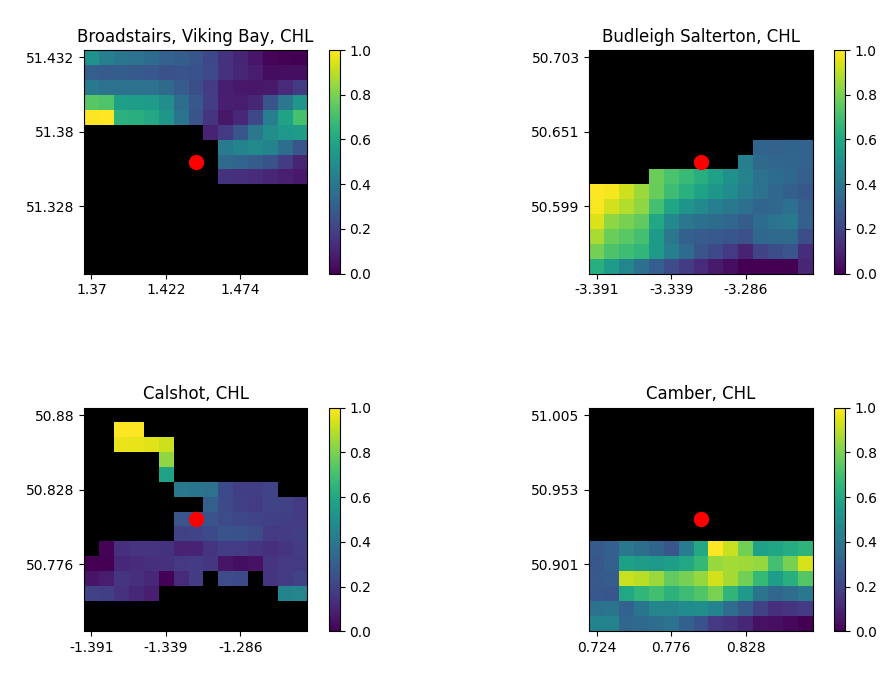
\includegraphics[scale=0.7]{images/2d_plots_chl.png}
    \caption{Selected 15x15 CHL Plots with pixel size of 1km x 1km. Black squares indicate spatial gaps for CHL, and for these few plots, it seems likely to be squares that are on land. Brighter coloured squares indicate a higher level of CHL. }
    \label{fig:selected15x15chl}
\end{figure}

It can be observed that almost all of the sites have some gaps in data spatially. Upon closer inspection, this seems likely because many sites are extremely close to land, such that the missing values are of points that are on land. Most of the red dots are also on black squares, meaning the point on the grid closest to the actual site is also a spatial gap. The colours on the graph, representing CHL levels, seem to change in a somewhat gradient manner, suggesting that there is a higher correlation in the CHL values of points closer to one another. Similar observations were found in the plots for the other 5 features.

Furthermore, note that for Budleigh and Camber, it appears that as we move further away from the coast, i.e. looking at squares closer to the edge (bottom in this case) of the plot, the squares become of a darker colour, indicating that CHL decreases. Whether this phenomenon is common across plots is difficult to observe from glancing at the plots. This motivates our use of feature engineering to aggregate over plots and examine how average values change as window size increases, as presented in section 2.3. 

In an attempt to see whether the points with colour change over time, such that it may suggest changing coastlines due to tidal shifts (where some areas are above water level at low tides but underwater at high tides), two days of data with one in July and one in March overlaid with each other in figure \ref{fig:coastline_shift}. Grey or orange squares indicate that across the two dates, the point is either both present in the dataset or both missing and red indicates otherwise. Red squares indicate that there are discrepancies across the two dates, such that on one of them that point is missing while on the other it is not. Perhaps due to the relatively lower resolution of the data, no obvious intertidal zones were observed. It was found that data availability for a window either remained constant throughout the two periods, or there was some data for one period and none at all for another period. Given that each window has a dimension of 15km, it does not appear that this can be caused by a coastline shift. Instead, it appears that a singular point's data availability changes and fluctuates vastly across time, perhaps due to the way that the satellite captures data. This motivates more investigation into missing values in the dataset before proceeding into model construction. 

\begin{figure}[H]
    \centering
    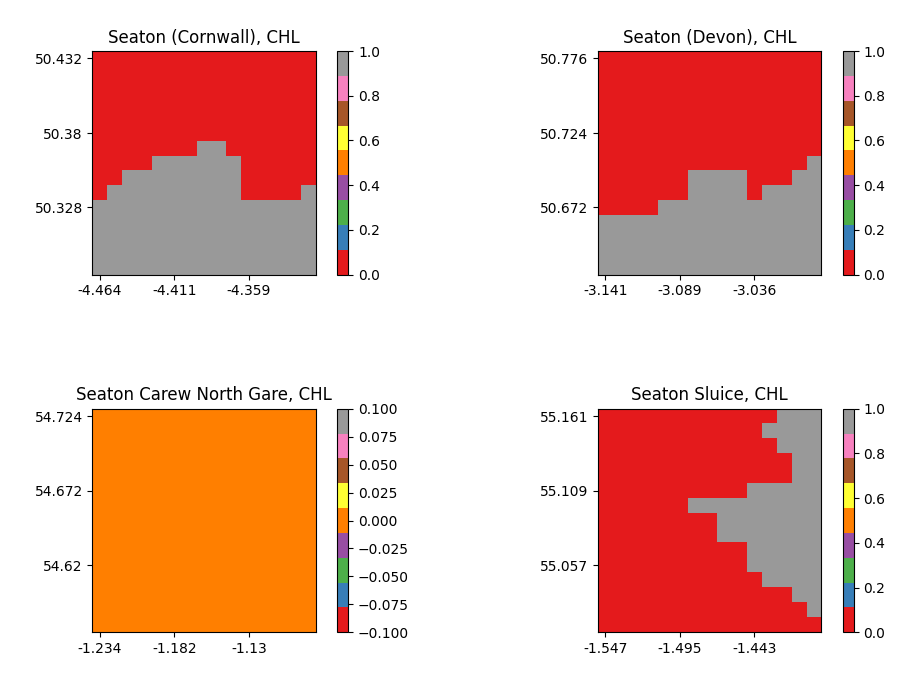
\includegraphics[scale=0.7]{images/2d_plots_difference.png}
    \caption{Comparing data availability across two dates. On plots with red and grey squares, red squares indicate that there are discrepancies in data availability over two time periods on these squares, while grey squares indicate that there are no discrepancies (e.g. this point is missing at both dates). Fully orange plots indicate there are no discrepancies in data availability over the two dates. }
    \label{fig:coastline_shift}
\end{figure}

\subsection{Visualising Missing Values}

Missing values exist on three dimensions: across time, across sites and spatially for each time-site pair. Missing values across time are first displayed in figure \ref{fig:missingdatas3time}. Each block represents data for a year, where each day has a number that indicates the number of sites with missing data on that day. A site is considered missing if for that day there are no values within any points in the 15 $\times$ 15 window of that site. A darker colour indicates a higher number of missing sites for the date.

\begin{figure}[H]
  \centering
  \caption{Missing Data Across Time. Each block represents data for a year, where each day has a number that indicates the number of sites with missing data on that day (missing data = no values within the 15 $\times$ 15 window for that site). Darker colour indicates a higher number of missing sites for the date.}
  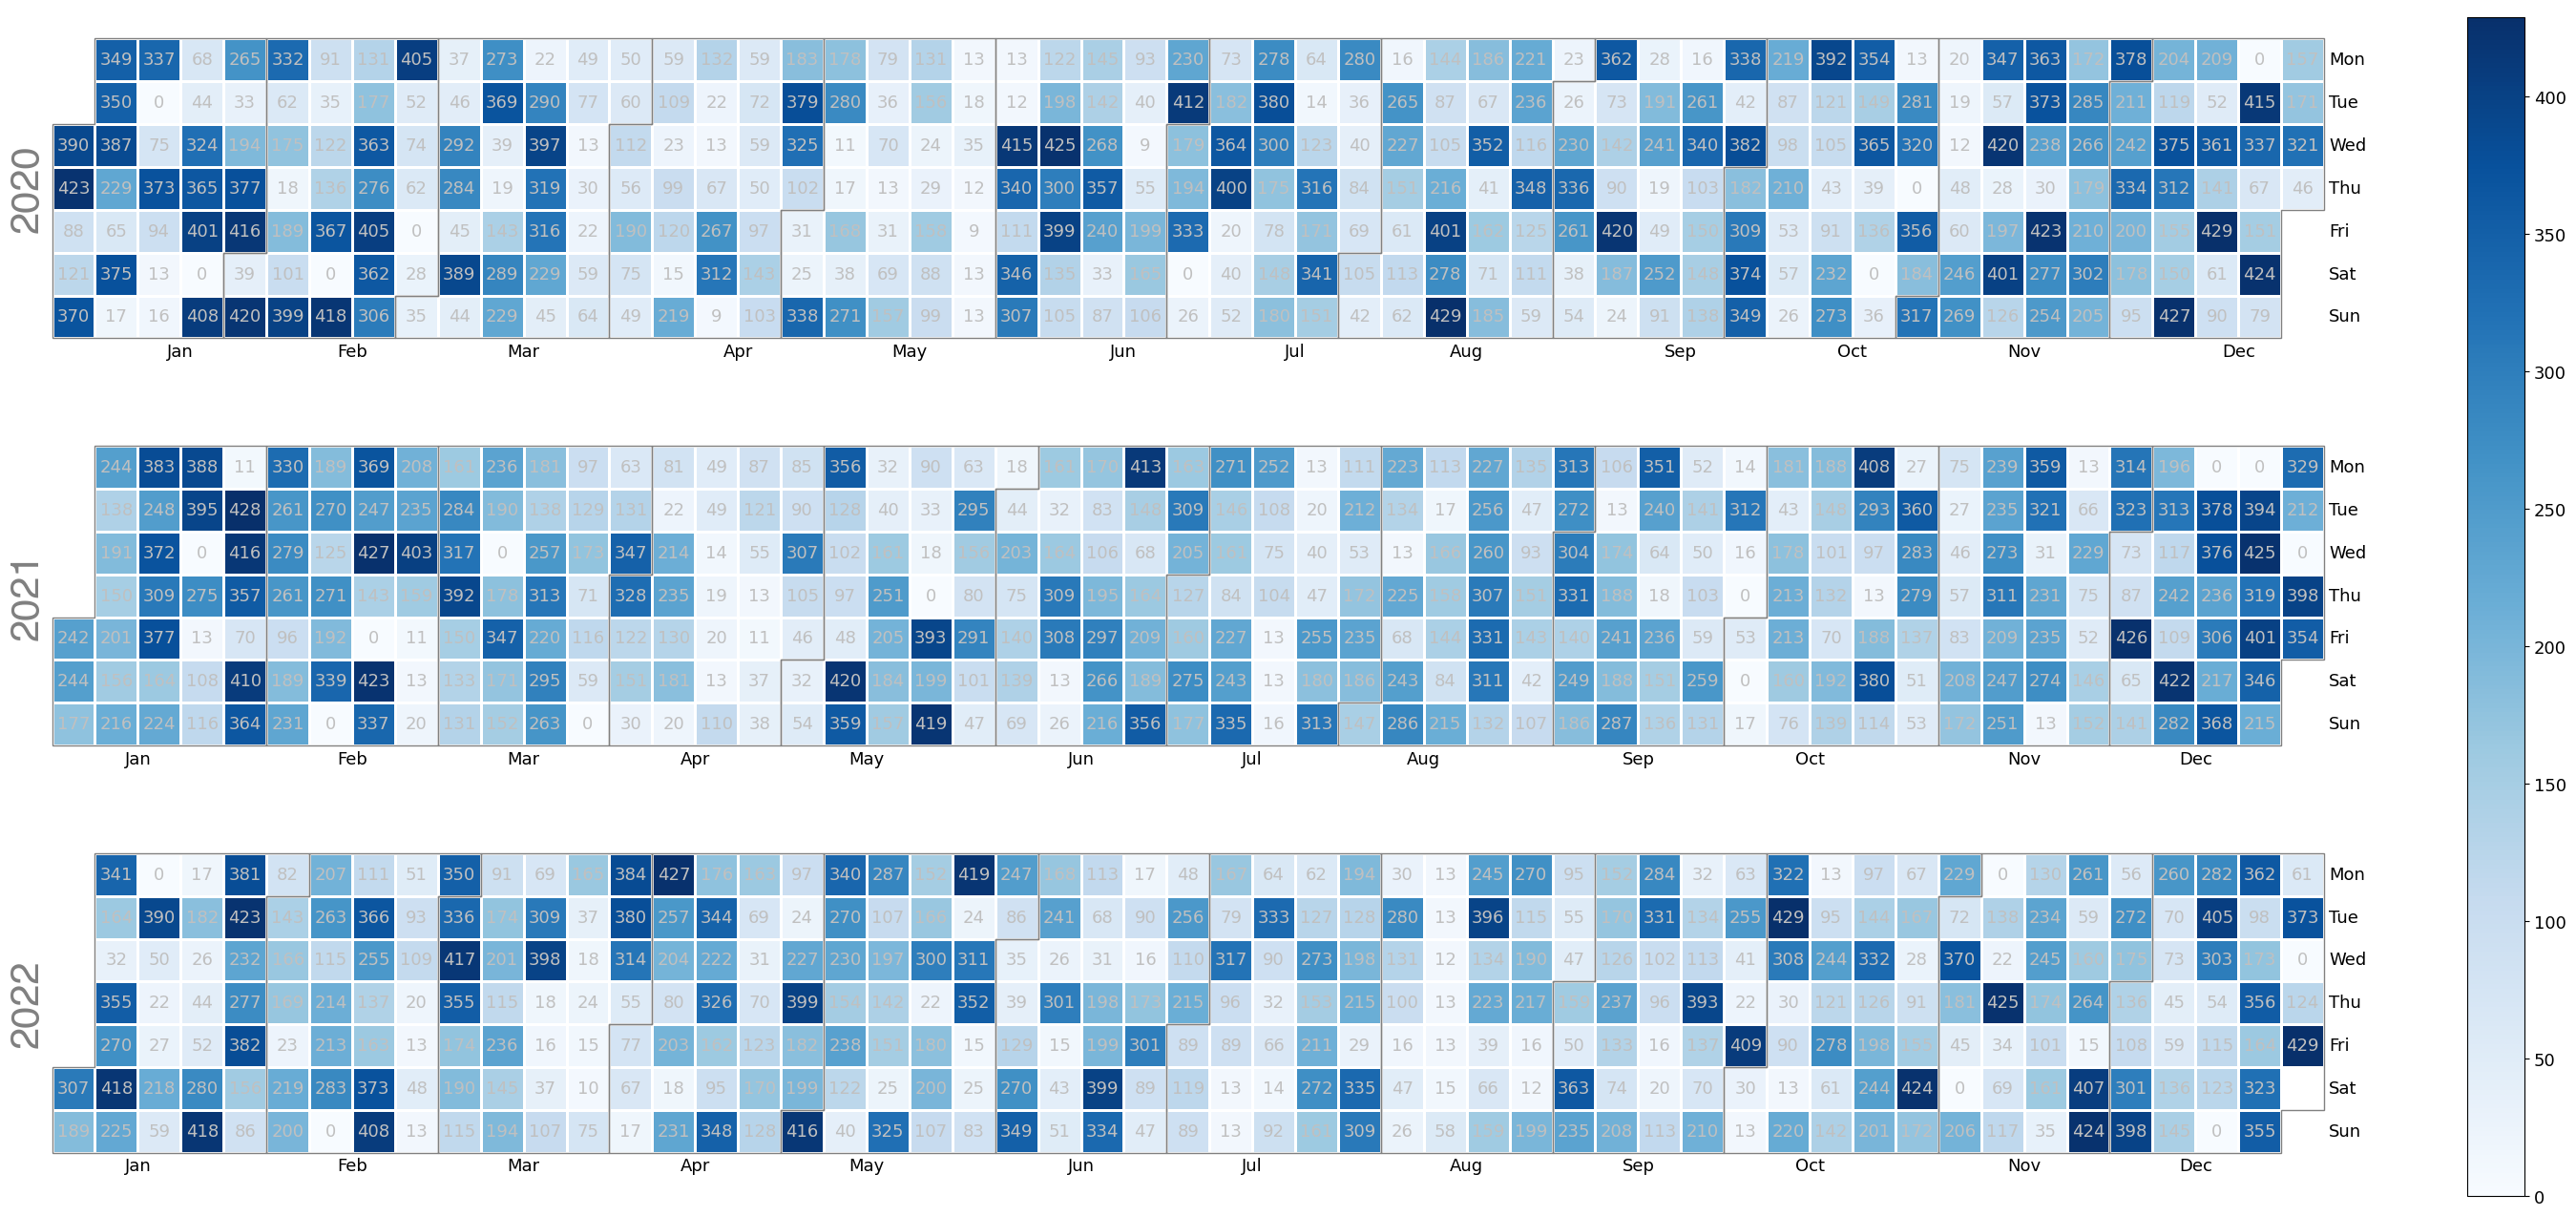
\includegraphics[width=\textwidth]{images/missing_values_s3_time.png}
  \label{fig:missingdatas3time}
\end{figure}

It can be observed that the data is more sparse in the winter months, i.e. from November to February, likely due to weather conditions, from the darker colours of the dates around then. There is also significant variability in data availability across days, likely also due to variable weather conditions. The data points that are available are likely from sites and dates where there are minimal clouds. 

Figure \ref{fig:missingdatas3site} presents the missing data across the dimension of the site in a histogram, with the horizontal axis depicting the number of missing days of data over three years (a total of 1096 days), and the vertical axis depicting the frequency of sites with the specified amount of missing data. 

\begin{figure}[H]
  \centering
  \caption{Missing Data Across Sites. X-axis is the number of missing days of data over 2020-2022. Y-axis is the frequency of sites with the specified amount of days missing data. We can see that most sites have a similar amount of days with missing data.}
  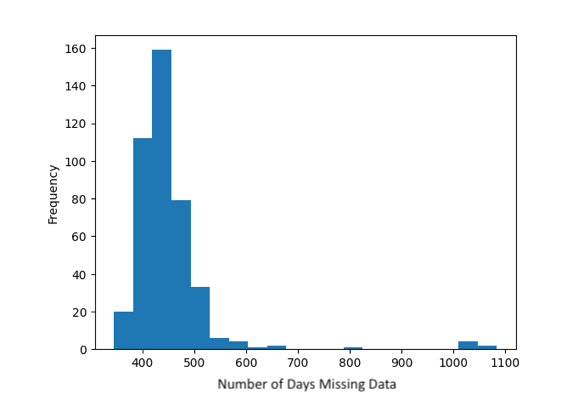
\includegraphics[width=250pt]{images/missing_values_s3_sites.png}
  \label{fig:missingdatas3site}
\end{figure}

It can be observed that most sites have a similar amount of missing data across the three years with the median to be around 450 days. This shows that despite there being more variability in missing data across time, missing data across sites are more comparable and thus it is still reasonable to treat different sites as being similar (close to identical) to each other in our models and analysis. 


\section{Engineered Features Data}
\subsection{Feature Engineering}

Our decision to engineer features in order to describe the geographic sites of interest for our further analysis is twofold. Firstly, as evident from preliminary 2D plots performed on the dataset (figure \ref{fig:selected15x15chl}), it was difficult to draw conclusions about whether some patterns observed for certain plots were also evident in other plots, and how common the occurrence of these patterns are, due to the large number of plots we have. Hence, to perform a numerical analysis of such patterns, the raw satellite images need to be described and summarised with some descriptive statistics. Secondly, engineering features would enable us to run more models in a more meaningful manner, enhancing the predictive modelling process. We are hoping to use satellite imagery as an input to machine learning models, and although some models (namely CNNs) are effective at extracting signals from raw images, other methods are not as effective and require manual feature engineering steps to be performed. 

Engineering features involved computing aggregated statistics — specifically, the mean, median, first quartile (q1), and third quartile (q3) — across various grid sizes for each data point. These aggregated statistics were computed for grid sizes ranging from 1x1 to 15x15, with an increment step of 2; that is, grids of sizes 1x1, 3x3, ..., 15x15. As a result, this produced 192 features (4 statistics x 8 grid sizes x 6 features) for each time and site pair.

The methods were applied to create datasets with the extracted features capturing the statistical relationships across each grid dimension. In subsequent analyses, these datasets were used to train several predictive models. The performance of the models trained on these new datasets will be compared and contrasted to assess the predictive power of the model, the most effective approach to handling missing values and to evaluate the benefits of the proposed feature engineering technique.


\subsection{Exploratory Data Analysis on Engineered Features}

An extensive set of features was created and analyzed to understand their characteristics and relationships.

\subsubsection{Comparison of Feature Values Across Grid Sizes}

The initial analysis aimed to explore the mean values of the engineered statistics (q1, q3, mean, and median) across grid sizes ranging from 1x1 to 15x15. This exploration was conducted on the dataset with engineered features without handling missing values. Figure \ref{fig:fea} displays how each feature's statistics change with different grid sizes.

In general, all the features exhibit greater variability as the grid size increases. This is evident from the widening gap between the q1 and q3 statistics, as well as between the median and mean, as the grid size grows. Such observations suggest that data becomes more diverse when analyzing the status from larger grids. With aggregation over an expanded geographic area, there's a higher probability of encountering time-site pairs with distinct characteristics or anomalies.

As the grid size expands, the values of all statistics for BBP, CDM, KD490, and CHL tend to decrease. This suggests that as one moves further from the shore, there are fewer particles in offshore waters, reduced absorption ability, less attenuation of light, and less aquatic vegetation. For SPM, most statistics decrease with increasing grid size, except for q3, which suggests that waters closer to the shore might contain more suspended matter. The variability of its value is greater than that of the previously mentioned four features, possibly due to local disturbances.

In contrast to other features, the statistical values of ZSD increase as the grid size expands. This indicates that the farther measurements are taken from the shore, the clearer the water becomes. However, note that the depth of the water could also impact value of ZSD. ZSD values are limited by the depth of the water column, and thus going further from the shore means deeper waters and thus a higher possible range of ZSD. 

The median and mean curves for each feature align closely. BBP and ZSD, in particular, almost entirely overlap. This might suggest a relatively symmetric distribution of BBP and ZSD values across different grid sizes. The relationships between various features will be analyzed in the subsequent section.


\begin{figure}[H]
  \centering
  \centering
    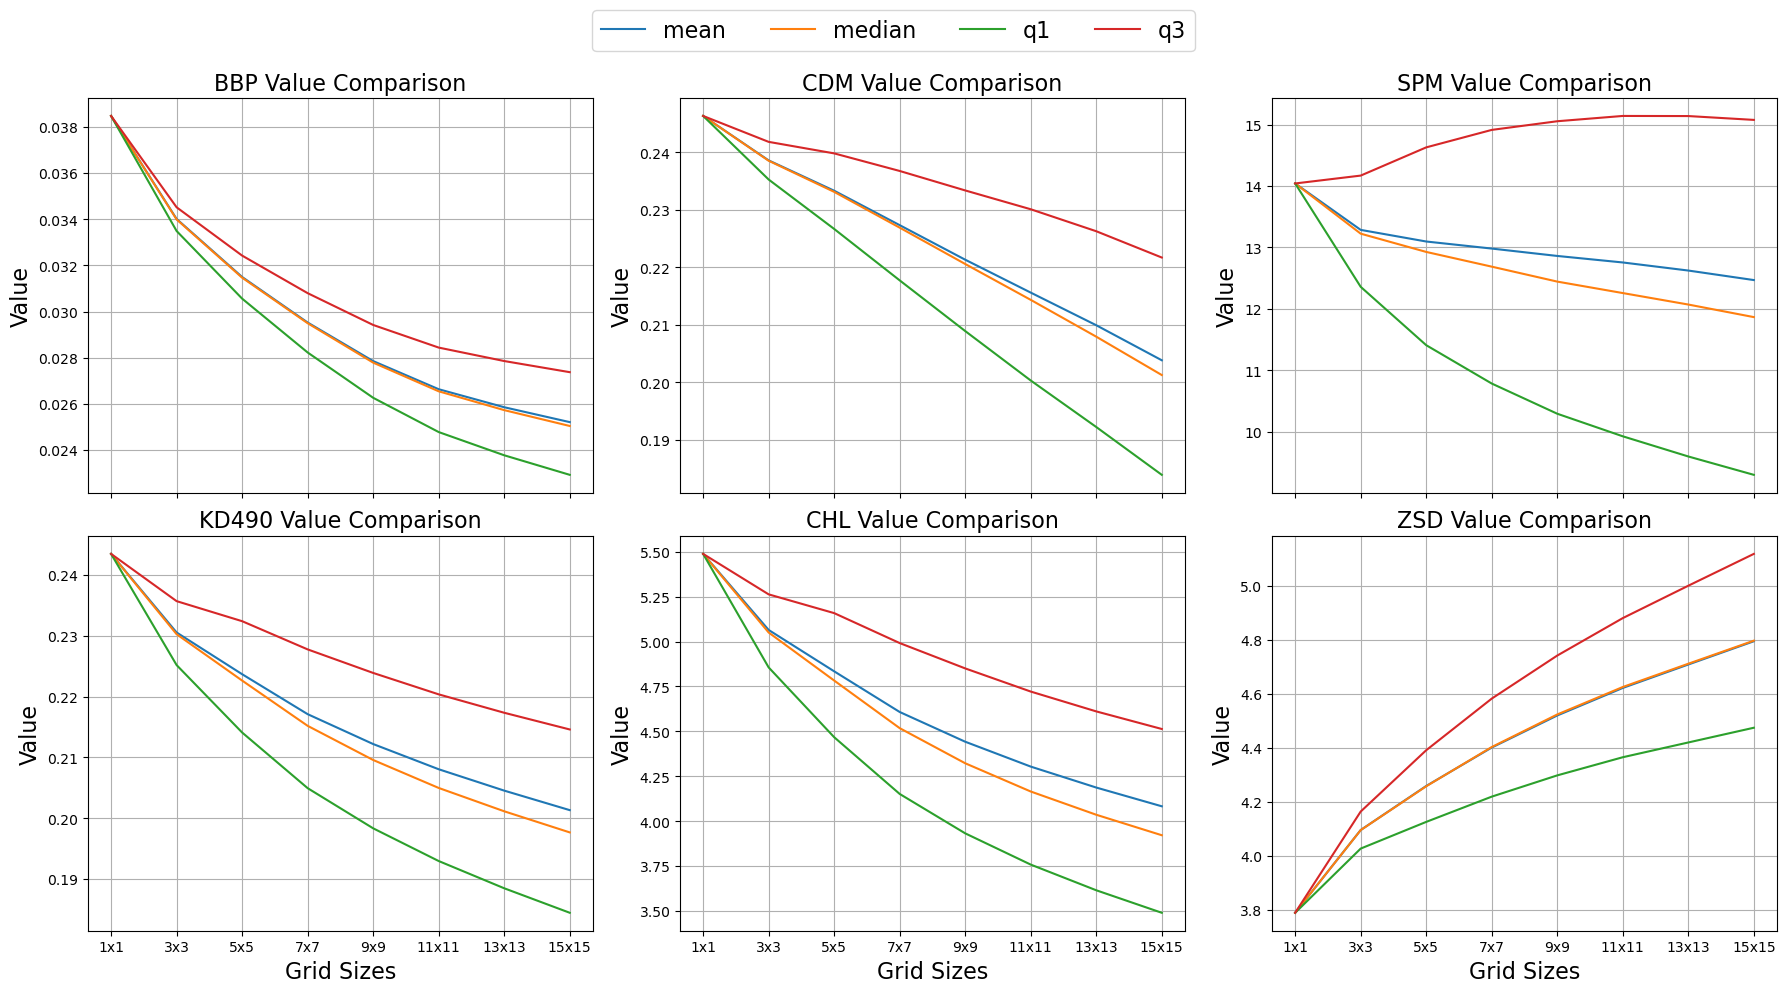
\includegraphics[width=\linewidth]{images/feature_na_eda.png}
    \caption{Feature Value Comparison Across Grid Sizes for Different Statistics}
    \label{fig:fea}

\end{figure}

\subsubsection{Correlation between Features and Risk Level}

After combining the datasets with risk level labels, the relationship between the engineered features and these risk levels was analyzed. The primary objective was to identify features that could significantly influence risk compared to the raw dataset(without feature engineering). 

The correlations between features and 'riskLevelLabel' were determined using Pearson's correlation coefficient, which evaluates the linear relationship between variables. This coefficient provides a value between -1 and 1 where a value close –1 or +1 indicates a strong linear relationship between two variables, and 0 indicates no linear relationship\citep{pearson}.

For each feature and grid size, the highest absolute correlation for each group was selected based on its absolute value and is presented in Table \ref{table:combined_corrs}. It is evident that certain features, such as SPM, are potentially more influential in predicting the risk level label compared to others. 

Furthermore, smaller grid sizes generally exhibit stronger correlations with risk levels. The 5x5 and 7x7 grid sizes also display a notably high correlation. This implies that a modest increase in grid size might capture valuable information. However, if the grid size becomes too large, the values tend to converge and lose their capability to represent the relationship with pollution risks effectively.

\begin{table}[h]
\centering
\begin{subtable}[c]{\textwidth}
\centering
\begin{tabular}{cccccc}
\toprule
\textbf{BBP} & \textbf{CDM} & \textbf{SPM} & \textbf{KD490} & \textbf{ZSD} & \textbf{CHL} \\ \midrule
 0.03571 & -0.02882 & 0.06684 & 0.01354 & -0.01157 & -0.01225 \\ \bottomrule
\end{tabular}
\caption{Correlations by Feature}
\label{tab:feature_corrs}
\end{subtable}
 
\vspace{5mm}           

\begin{subtable}[c]{\textwidth}
\centering
\begin{tabular}{cccccccc}
\toprule
\textbf{1x1} & \textbf{3x3} & \textbf{5x5} & \textbf{7x7} & \textbf{9x9} & \textbf{11x11} & \textbf{13x13} & \textbf{15x15} \\ \midrule
0.06684 & 0.05673 & 0.05826 & 0.05872 & 0.05717 & 0.05535 & 0.05300 & 0.05225 \\ \bottomrule
\end{tabular}
\caption{Correlations by Grid Size}
\label{tab:gridsize_corrs}
\end{subtable}

\caption{Summary of Highest Correlations with Risk Level Label}
\label{table:combined_corrs}
\end{table}

The features with mean statistics and the 7x7 grid were specifically examined to assess the effectiveness of the feature engineering in reflecting correlations since it has the highest correlation with 'riskLevelLabel', except for the smallest grid size for sites, 1x1.

While the Pearson correlation coefficients offer valuable insights into the relationships, it is evident that the correlations aren't exceptionally high. This moderate correlation could be attributed to the fact that our target variable, the 'riskLevelLabel', is binary. In such settings, using visualization techniques like boxplots might offer more intuitive insights into the relationship between features and risk level. Box plots of all 6 features from the original dataset (\ref{fig:rawbox}) and the 7x7 mean features from the engineered dataset (\ref{fig:15box}) were plotted against the 'riskLevelLabel'. From boxplots of 7x7 mean features with 'riskLevelLabel' shown in \ref{fig:15box}, it is evident that high values of BBP and SPM are more likely to appear as pollution risk increases. The levels of CHL and KD490 tend to be higher in general with increased risk, while levels of ZSD tend to be lower. The variability of CDM is even higher when pollution risk is at a normal level.

\begin{figure}[H]
\centering
\captionsetup{width=.9\linewidth}
\begin{subfigure}[c]{\textwidth}
    \centering
    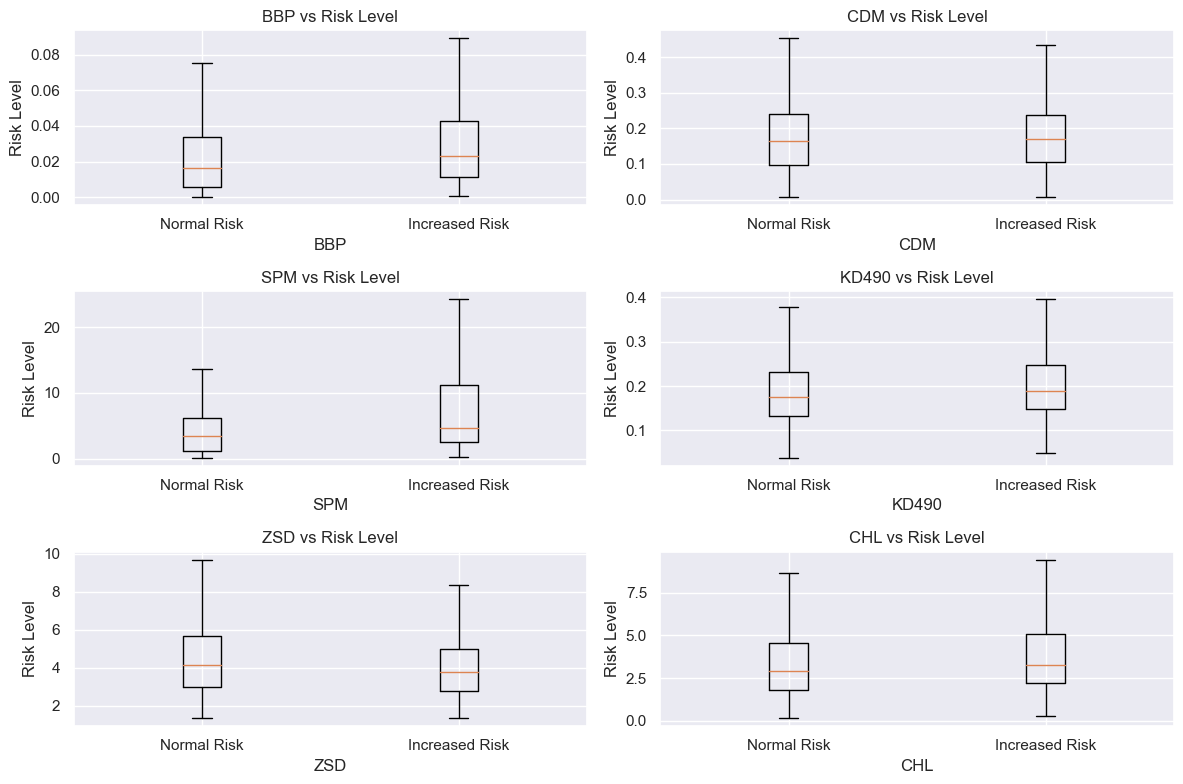
\includegraphics[width=\linewidth]{images/raw_boxplot.png}
    \caption{Features with 'riskLevelLabel' for Original Data (Without Feature Engineering)}
    \label{fig:rawbox}
\end{subfigure} \\
\vspace{5mm}      

\begin{subfigure}[c]{\textwidth}
    \centering
    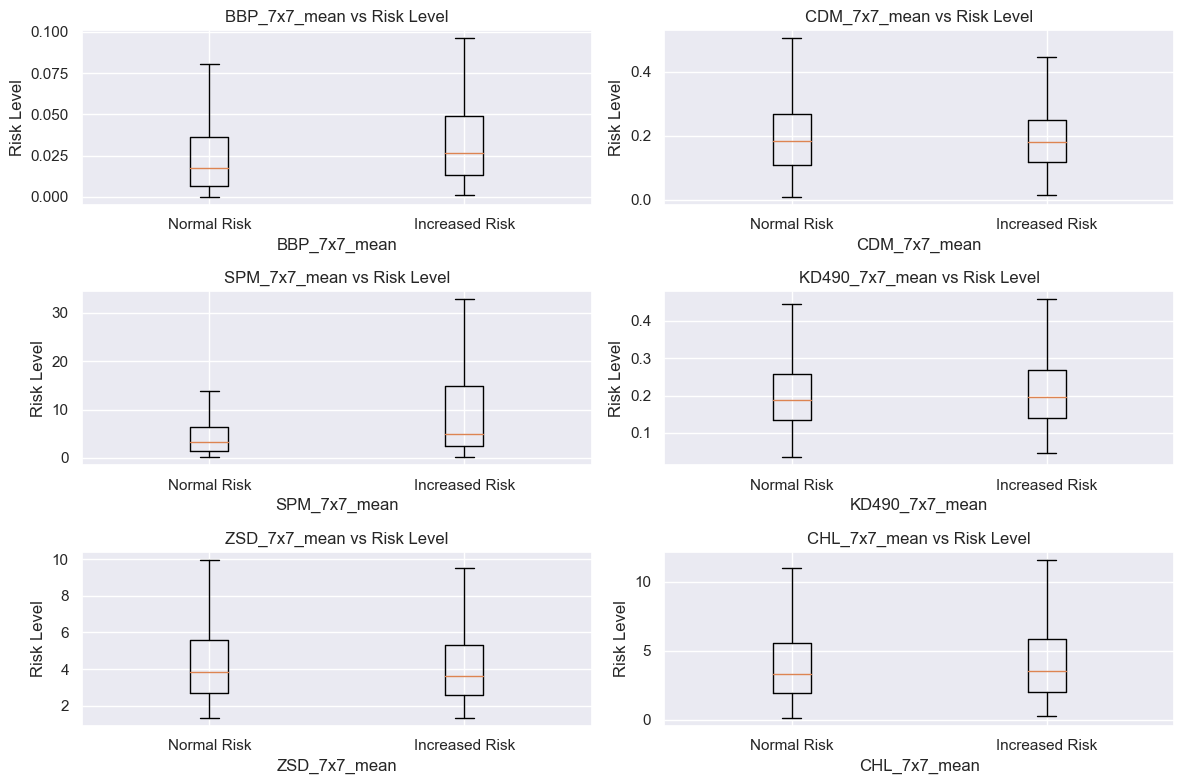
\includegraphics[width=\linewidth]{images/7x7_mean_boxplot.png}
    \caption{7x7 Mean Features with 'riskLevelLabel' (Feature Engineered Dataset)}
    \label{fig:15box}
\end{subfigure}

\caption{Boxplots comparing the correlation between features in the raw dataset and feature-engineered dataset (7x7 Mean)}
\end{figure}


By comparing the pair plots of all features from the original dataset (\ref{fig:pair}) to the 7x7 mean features (\texttt{BBP\_7x7\_mean}, \texttt{CDM\_7x7\_mean}, \texttt{SPM\_7x7\_mean}, \texttt{KD490\_7x7\_mean}, \texttt{ZSD\_7x7\_mean}, and \texttt{CHL\_7x7\_mean}) from the engineered dataset (\ref{fig:15pair}), it is evident that the overall correlations between features remain similar. CHL and KD490 exhibit an almost linear positive correlation, while ZSD shows a negative correlation with both KD490 and CHL. This observation is consistent with research indicating that KD490 and ZSD can be expressed as functions of CHL and therefore highly correlated \citep{MOREL200769}. However, no strong correlation can be observed between the predicted risk (represented with blue and orange legends) and any of the features in the pair plots.

\begin{figure}[H]
\centering
\captionsetup{width=.9\linewidth}

\begin{subfigure}[c]{0.45\textwidth} % Adjust width to slightly less than 0.5 to accommodate any spacing/margin between subfigures
    \centering
    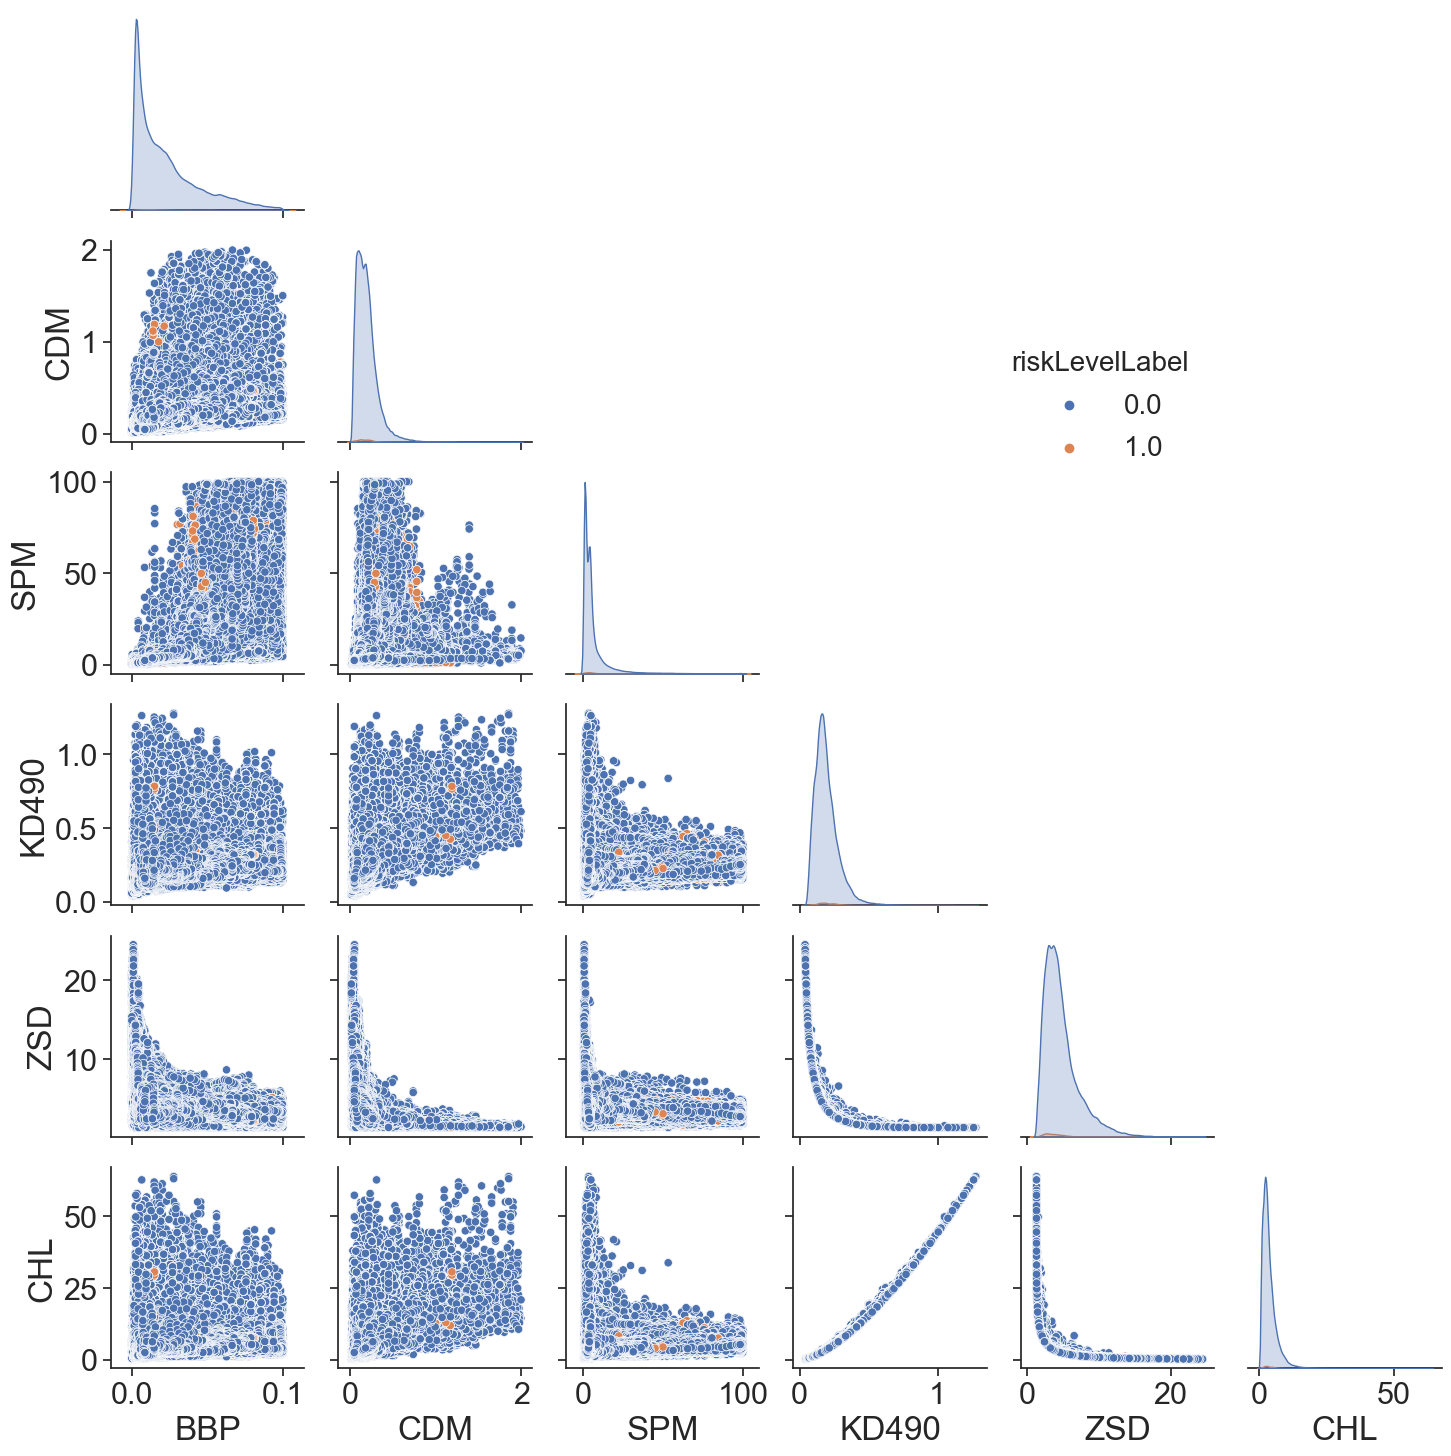
\includegraphics[width=\linewidth]{images/original_pairplot.png}
    \caption{Features for Original Data (Without Feature Engineering)}
    \label{fig:pair}
\end{subfigure}
\hfill % This will ensure that the two subfigures are spaced apart as far as possible within the line
\begin{subfigure}[c]{0.45\textwidth} % Adjust width to slightly less than 0.5 to accommodate any spacing/margin between subfigures
    \centering
    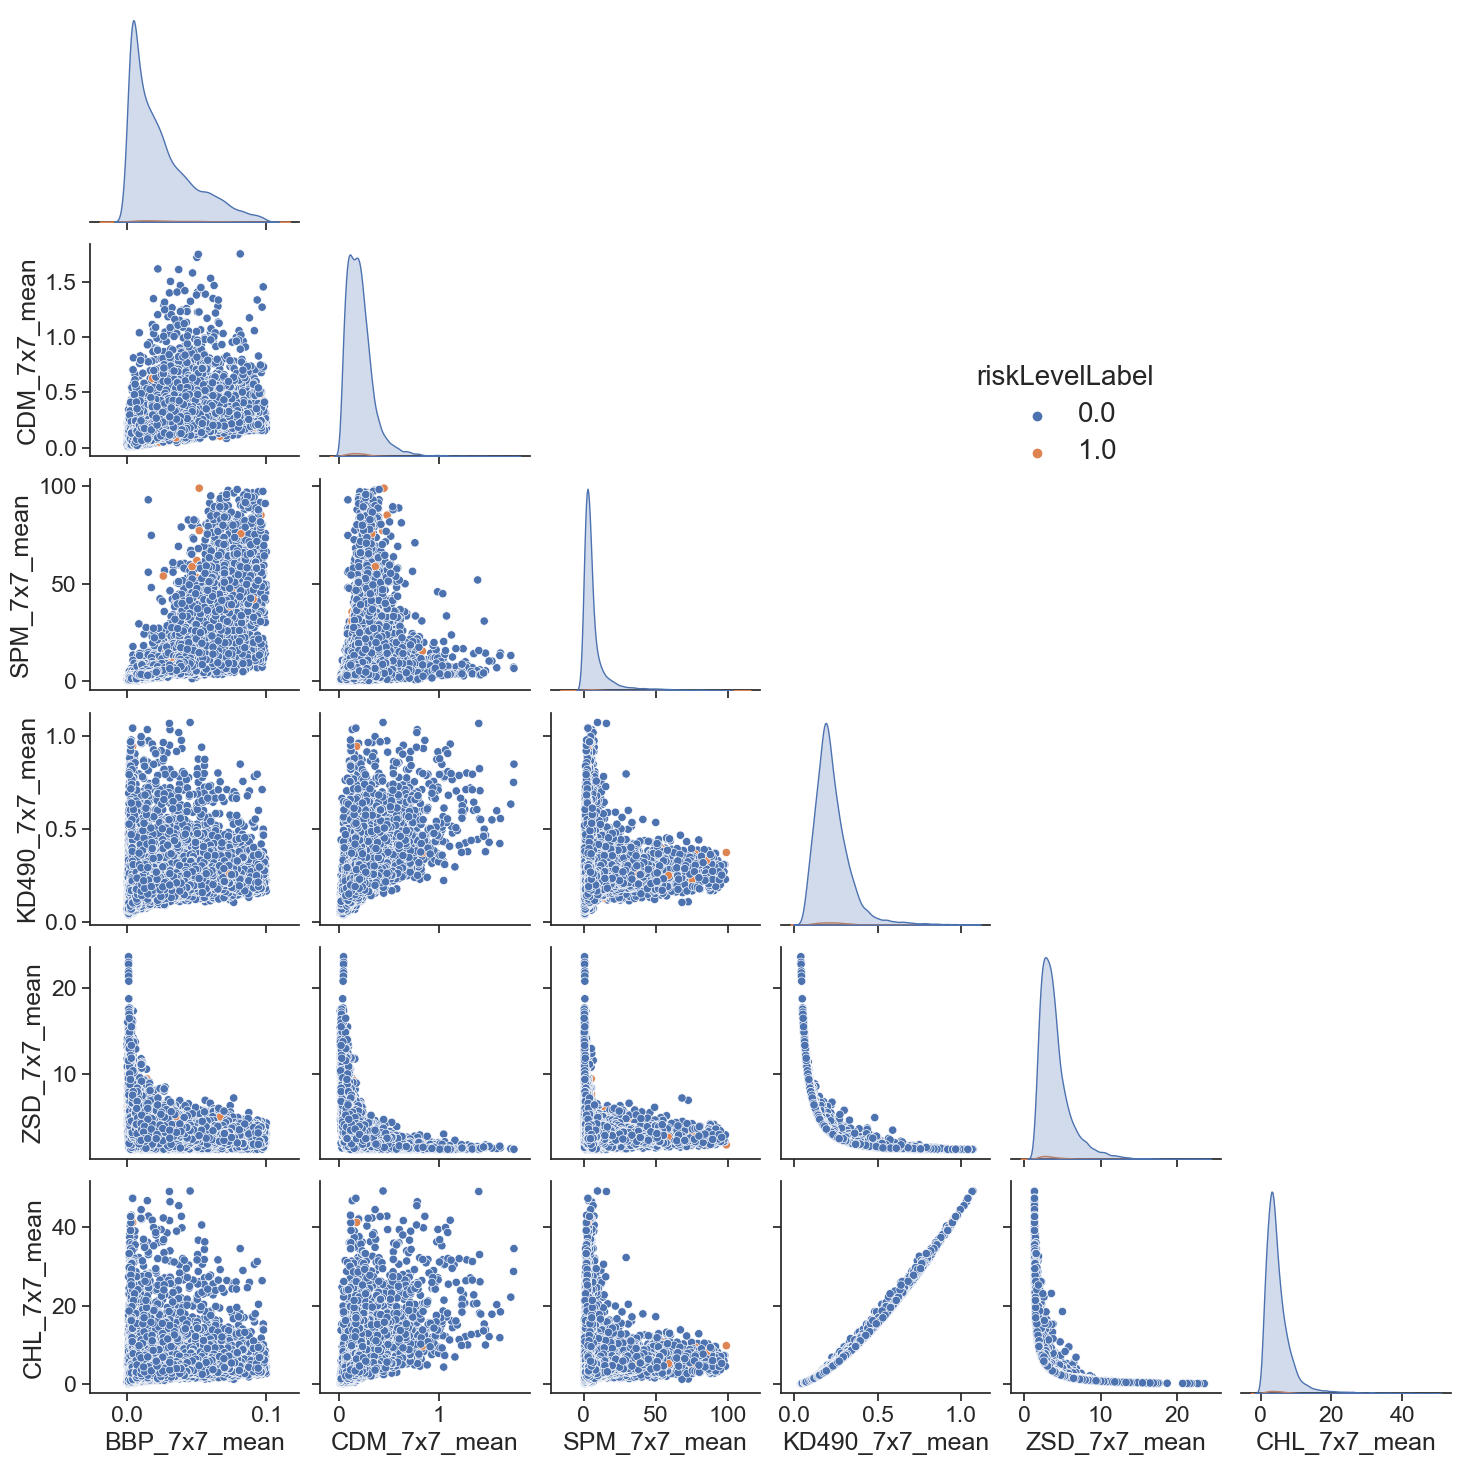
\includegraphics[width=\linewidth]{images/7x7_mean_pairplot.png}
    \caption{7x7 Mean Features (Feature Engineered Dataset)}
    \label{fig:15pair}
\end{subfigure}

\caption{Pairplots comparing the correlation between features in the raw dataset and feature-engineered dataset (7x7 Mean)}
\end{figure}


However, the simple linear correlations may not wholly capture the complex interplay between these variables and the pollution risk level. Fusing all these factors through machine learning models could potentially unravel the complex relationships and provide a more accurate representation, which allows us to continue exploring using machine learning methods in the subsequent section \ref{sec:predictive}.



\begin{comment}
   \begin{figure}[h]
  \centering
  \centering
    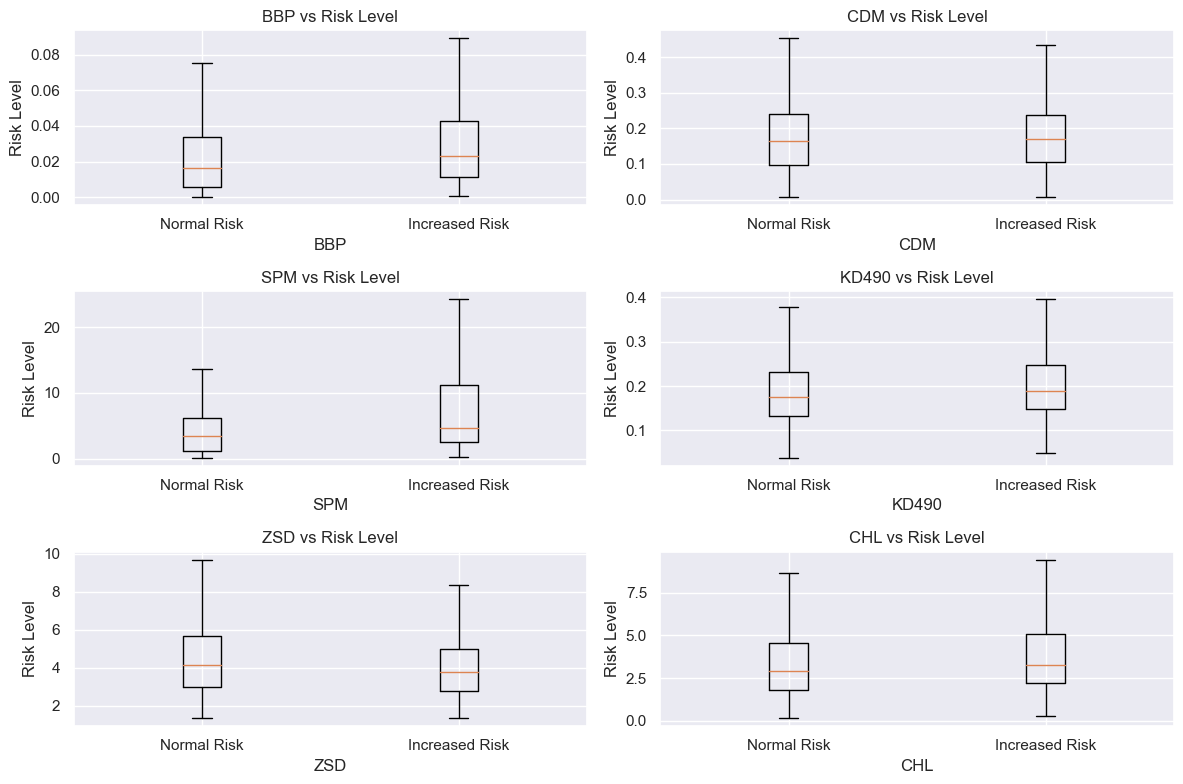
\includegraphics[width=0.8\linewidth]{images/raw_boxplot.png}
    \caption{Boxplot of All Features with riskLevelLabel for Raw Data (Without Feature Engineering)}
    \label{fig:rawbox}
\end{figure}

\begin{figure}[h]
  \centering
  \centering
    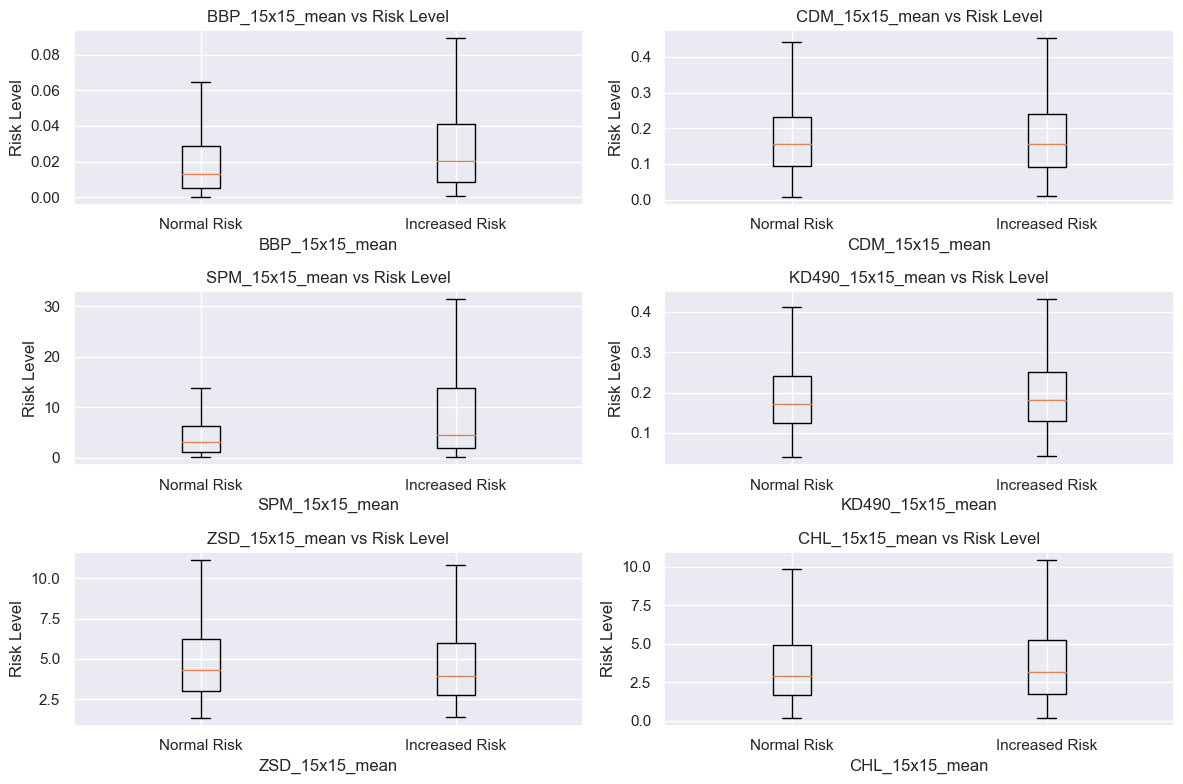
\includegraphics[width=0.8\linewidth]{images/15x15_boxplot.png}
    \caption{Boxplot of 5x5 Median Features with riskLevelLabel (Feature Engineered Dataset) \qs{to be updated}}
    \label{fig:15box}
\end{figure} 
\end{comment}

\subsection{Clustering Analysis on risk-level-increased data}
\label{sec:clustering}
In this part, we looked into the risk-level-increased data only, and trying to measure the heterogeneity among them. This analysis will help us better characterize different kinds of risk-level-increased data before trying various predictive models.

We used K-Means to conduct our clustering analysis with the mean of six features (BBP, CDM, SPM, KD490, ZSD and CHL) for a window size of 15x15. In order to prevent the missing values from interfering with the K-means clustering, we only kept the samples without any missing values. To ensure no feature dominates the clustering and get more straightforward insight, Z-Score transformation was applied on the risk-level-increased data with mean and standard deviation of risk-level-normal data, i.e. $ X_{1 \text{\_scaled}} = \frac{X_{1} - \text{mean}(X_{0})}{\text{std}(X_{0})}$.

Figure \ref{fig:K_Elbow} is the Elbow Curves \citep{kodinariya2013review}, which is the WCSS (Within-Cluster Sum of Square) against different numbers of clusters. In order to find the 'elbow' point of the graph, the silhouette method is applied. The idea of silhouette method \citep{kodinariya2013review} is to calculate the silhouette coefficient of each data point, that is 
\begin{equation}
s(i) = \frac{b(i) - a(i)}{\max\{a(i), b(i)\}}
\end{equation} 

where
\begin{itemize}
\item $a(i)$ is the average distance from the $i^{th}$ sample to the other samples in the same cluster. 
\item $b(i)$ is the smallest average distance from the $i^{th}$ sample to samples in a different cluster, minimized over clusters
\end{itemize} 

The average silhouette coefficient of every data point is the silhouette score. The value of this score ranges between -1 and 1, it reached peak at K = 2, which is 0.43. So risk-level-increased data was divided into 2 clusters. 

\begin{figure}[H]
  \centering
  \begin{minipage}{0.45\textwidth}
    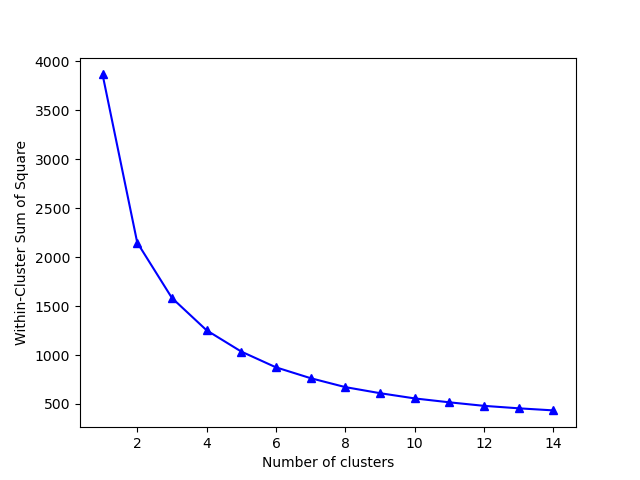
\includegraphics[width=\linewidth]{images/Kmeans_Elbow.png}
    \caption{The Elbow Curve}
    \label{fig:K_Elbow}
  \end{minipage}
  \hfill
  \begin{minipage}{0.45\textwidth}
    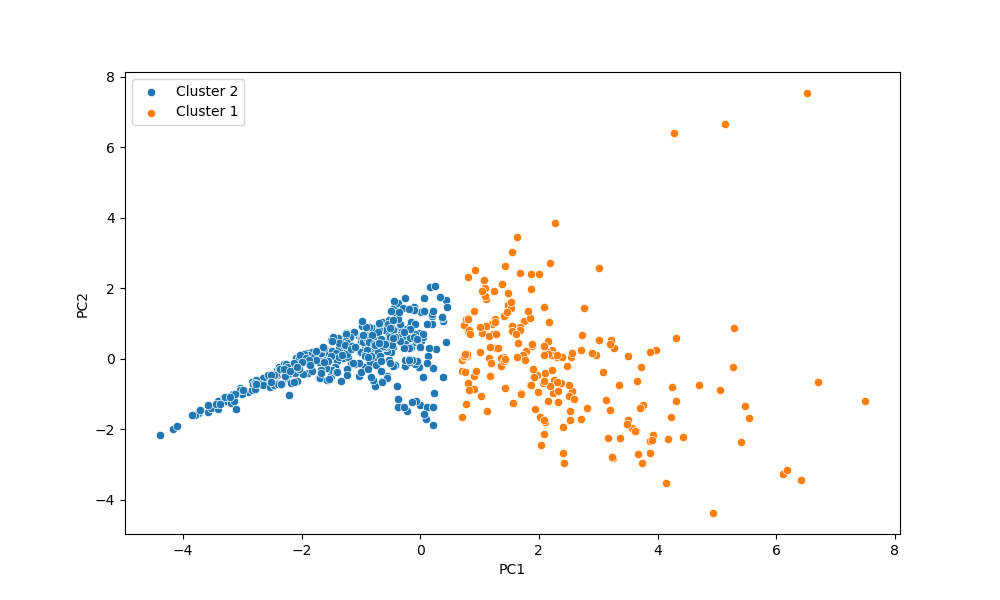
\includegraphics[width=\linewidth]{images/Kmeans_scatter.png}
    \caption{The Scatter plot for clusters}
    \label{fig:K_scatter}
  \end{minipage}
\end{figure}

The visual interpretation for both clusters is shown in Figure \ref{fig:K_scatter}, where all data points were distributed in a 2-dimensional space obtained by applying Principal Component Analysis. Furthermore, Figure \ref{fig:cluster_details} shows the distributions of six water quality indicators in each cluster. The values for the barplot were obtained by applying Z-score transformation (with mean and standard deviation of risk-level-normal data) on the mean of each feature's raw data.

\begin{figure}[H]
\begin{center}
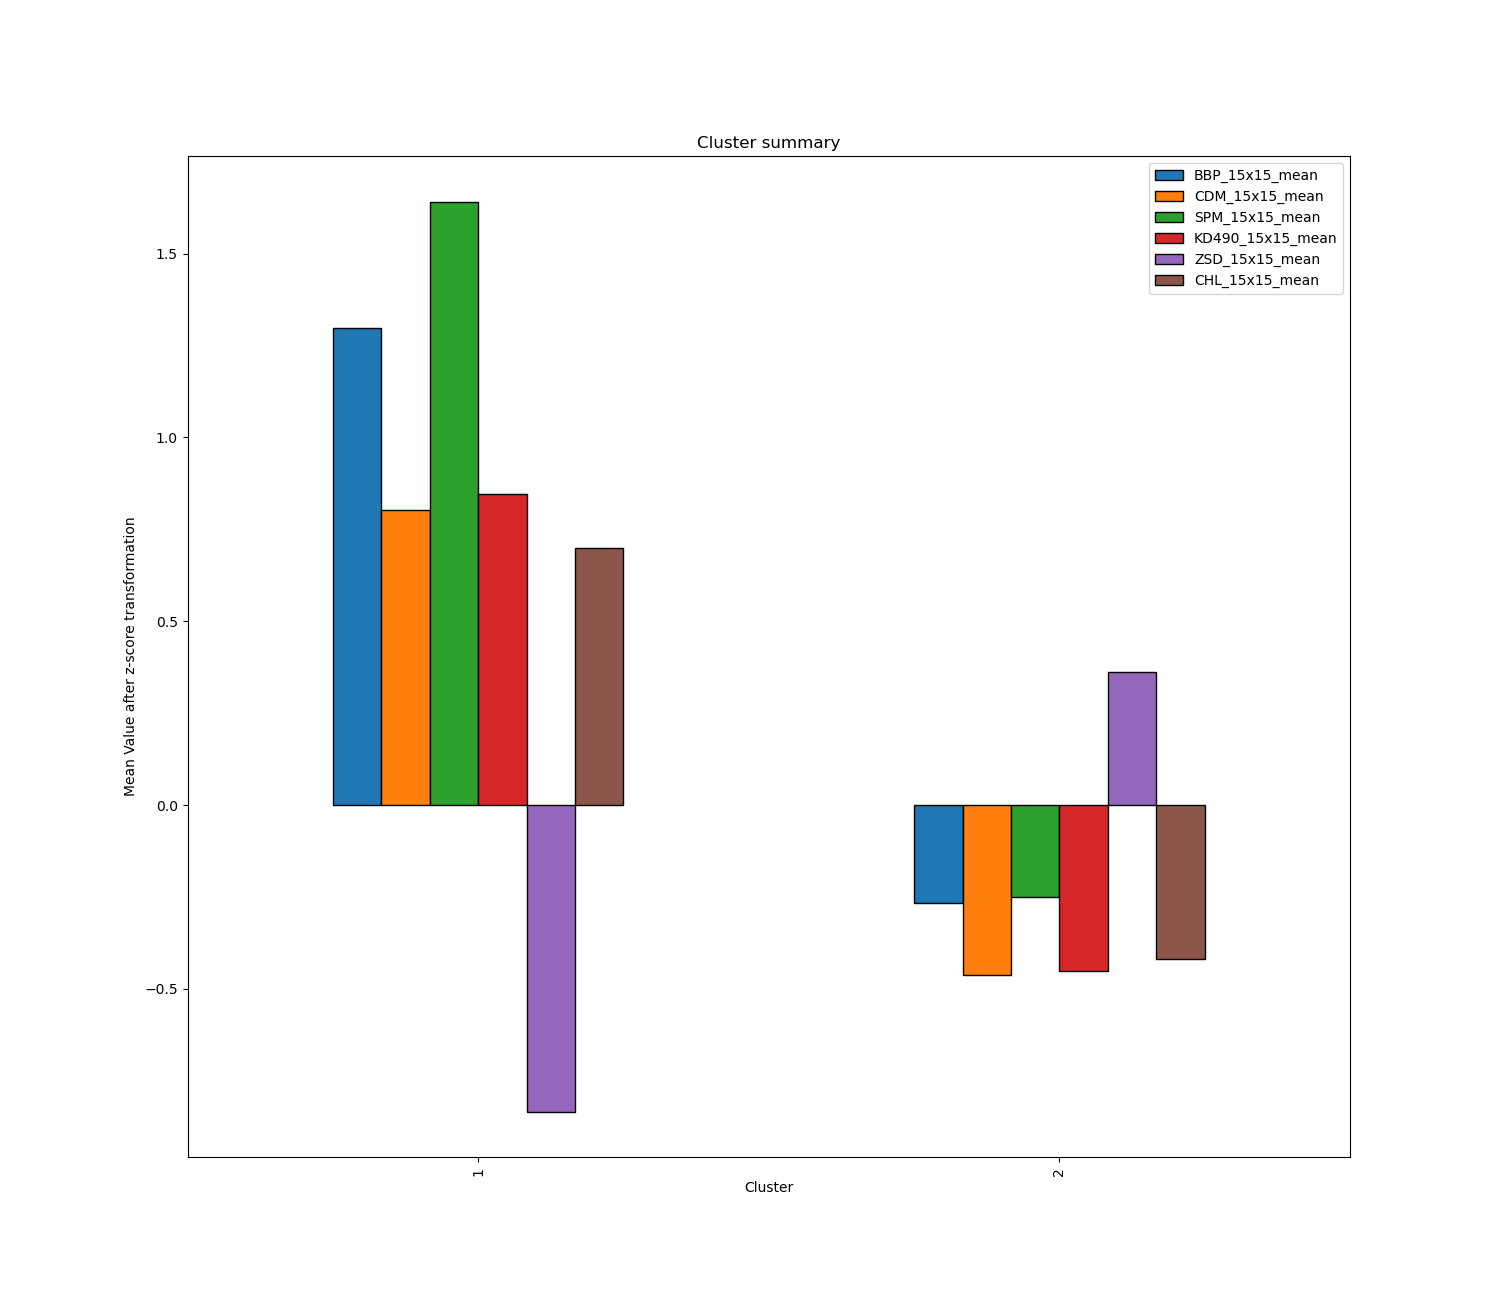
\includegraphics[width=1\linewidth, height=0.45\textheight]{images/Kmeans_cluster_detail.png}
\caption{Details in each cluster}
\label{fig:cluster_details}
\end{center}
\end{figure}

The risk-level-increased data was divided into two clusters. Cluster 1 contained 202 samples and cluster 2 contained 386 samples. Cluster 1 had high values of BBP, CDM, SPM, KD490 and CHL among the risk-level-normal data, especially for BBP and SPM, but ZSD is lower. Cluster 2 vice versa. For Cluster 1, nearly all five positive bars are above 0.75, which indicates the average values of these five features in this cluster are higher than almost 80\% samples from risk-level-normal data.

The performance between these two clusters for various models will be discussed in Section \ref{sec:across_clusters}.


\chapter{Methodology}

This section presents our methodology for investigating how satellite data can be used to make predictions about sewage pollution. The first section presents an overview of our methodology by formally presenting our main goal of building a binary classifier to predict sewage pollution and explains various lines of inquiry to explore the most important factors for building an effective classifier. The second section explains how missing data were handled in a standardized way before the data was fed into models. The third section details the numerous models trialled for building a binary classifier, explaining the motivations behind the architecture and settings for each model. The fourth section includes a brief comparison of computation gains from using principal component analysis. 

\section{Overview}

\textbf{Binary Classifier} \\
The main goal of the project was to build a binary classifier prediction model that aims to take satellite data as inputs and predict whether there is sewage pollution or not at a particular site for a particular date. We hope to trial various models for the binary classifier and find one that performs the best. The binary classifier prediction problem can be formalized by the following equation: 
 
$$ f_{t,s}: X_{t,s} \rightarrow \{0, 1\} $$ 
where $X_{t,s}$ refers to the variables from satellite data for date $t$ and site $s$, and $f_{t,s}$ refers to a binary classifier that predicts 1 if there is sewage pollution and 0 otherwise for a specific date $t$ and site $s$. This allows us to predict sewage pollution incidents $f_{t,s}$ for a site $s$ on a particular day $t$ using satellite data $X_{t,s}$ from that exact day. The reason we chose to do 'now-casting' was because satellite data from the same day is expected to show best whether there has been sewage pollution in that day.   

The classification was selected over regression for building our model due to the nature of the bathing water data, which provides categories for pollution rather than a numerical scale. The problem was further simplified to a binary classification task to simplify interpretation, as the other labels in the bathing water data do not further break down pollution very cleanly, and there are already much fewer positive samples for days and sites with sewage pollution. \\

\noindent \textbf{Dataset} \\
Based on exploratory data analysis performed in the previous section, the main dataset for model training and testing was created with an inner merge between the bathing water quality and the S3 satellite datasets, such that only time-site pairs that are non-missing in both datasets are used. S3 dataset was selected over S2 dataset as it contains more unique time-site pairs (table \ref{tab:s2_s3_comparison}). For the S3 data, a time-site pair is considered non-missing as long as there is at least one point in the 15x15 window for at least one feature for a time-site pair with a non-null value.

To find the best binary classifier, a structured training and testing approach was used to compare performance across multiple models. Each model would be trained on a fixed training dataset, where hyperparameters would be tuned with the help of a fixed validation dataset and the performance of the model evaluated on a fixed test dataset. The split would be 60/20/20 for training/validation/test and was done before training the models randomly. Table \ref{table:train_test_val} presents an overview of the train, validation and test datasets. 

\begin{table}[H]
        \caption{Overview of Train, Validation and Test Datasets on S3}
        \label{table:train_test_val}
        \centering
        \begin{tabular}{lcccc}
        \toprule
        \textbf{Dataset} & \textbf{Split \%} & \textbf{\# of Datapoints} &  \textbf{\# of Pos. Samples} & \textbf{\% of Pos. Samples} \\
        \toprule
        S3 Train & 60\% & 112,266  & 3,074 & 2.74\% \\
        S3 Val & 20\% & 37,422 & 1,083 & 2.89\% \\ 
        S3 Test & 20\% & 37,423 & 1,008 & 2.69\% \\ \midrule
        S3 & 100\% & 187,111 & 5,165 & 2.76\% \\ \bottomrule
        \end{tabular}
\end{table}

\noindent \textbf{Further lines of investigation} \\
Our initial numerical experiments compared performance across models in a standardised way, as was the initial aim of our project. While performing exploratory analyses on our datasets and running these experiments, we found more interesting questions to explore and more interesting ways to compare the models. Thus, we expand upon our investigations, such that the main investigative questions to be answered are: 

\begin{itemize}
    \item \textit{Which binary classifier performs the best on S3 data?} This is the main investigative question driving the project. We evaluated the results on 4 supervised learning models, where we trained and tested each on two separate datasets, totalling 8 binary classifiers. 
    \item \textit{What are the strengths and weaknesses of the best binary classifiers?} We hoped to investigate whether performance varies temporally (across months / years) or spatially (across regions in the United Kingdom) for the best binary classifiers of each model category, to better understand in what situation we would recommend usage of our binary classifiers. We also investigated whether the binary classifiers performed better on certain clusters of data (figure \ref{fig:cluster_details}). 
    \item \textit{How effective is the feature engineering approach in enhancing model performance?} With some models, we believe that data aggregation from feature engineering can enhance model performance, while with others using the raw data may be more beneficial. We hoped to test and evaluate these hypotheses comprehensively. 
    \item \textit{Does having a higher resolution, more fine-grained satellite dataset help with predicting sewage pollution?} More fine-grained result essentially means more data but would also potentially introduce more noise to the dataset. This was investigated by comparing S2 and S3 data, trimming them so they cover the same time-site pairs and approximately the same area. It is important to look at this question from a practical standpoint, as if this was true, we could get better model performance if the higher resolution Sentinel-2 could collect data more frequently.  
    \item \textit{How does the performance of our best binary classifiers fluctuate across spatial window sizes?} We expect to see performance increasing with window size up to a certain value, then decreasing from there onwards. We hope to test this hypothesis and observe whether there is an optimal window size for the models, as taking a larger window size comes at a higher computational cost. 
\end{itemize} 

These questions are each explored in sections \ref{sec:Comparison of Best Models}, \ref{sec:Strengths and Weaknesses of Best Models}, \ref{sec:Gains From Feature Engineering}, \ref{sec:Comparison between Sentinel 2 and Sentinel 3 Data} and \ref{sec:Impact of Window Size} respectively under numerical experiments, and shaped the main results and findings of this project. \\

\noindent \textbf{Evaluation Metrics} \\
The evaluation statistics used in this report are \(F1\text{-score}\), Precision, Recall, Average Precision (AP) and Area under the Receiver Operating Characteristic Curve (ROC\_AUC). The reason not to consider Accuracy is the highly imbalanced label, the accuracy could reach 94.5\% even with the baseline model. In this case, other metrics, such as the trade-off between precision and recall are more informative. Specifically, \(F1\text{-score} = 2 \times \frac{\text{precision} \times \text{recall}}{\text{precision} + \text{recall}}\) was used as the most important metric for evaluating models and as a criterion for hyperparameter tuning. 

\vspace{0.5cm}
\begin{minipage}{.25\textwidth}
\begin{tabular}{c|cc}
\hline
 & \textbf{True 1} & \textbf{True 0} \\ \hline
\textbf{Predicted 1} & True Positive (TP) & False Positive (FP) \\ 
\textbf{Predicted 0} & False Negative (FN) & True Negative (TN) \\ \hline
\end{tabular}
\end{minipage}%
\hfill
\begin{minipage}{.3\textwidth}
\centering
\textbf{Precision} \(= \frac{TP}{TP + FP}\) \\
\vspace{1em}
\hspace{1.5em}\textbf{Recall} \(= \frac{TP}{TP + FN}\)
\end{minipage}
\vspace{0.5cm}

The following sections explain the data pre-processing done to arrive at our model-ready datasets in more detail and explain the chosen models for the investigation. The models involve models that take in both the raw, windowed satellite data and engineered features.

\section{Handling Missing Data}

One of the primary challenges encountered in the dataset was the presence of missing data across various times, locations, and features. The missing values might be attributed to factors such as infrequent observations, cloud cover, and others. To address this issue, a two-step strategy for applying missing values was applied:

\subsection{Grouped Mean Substitution}

For each 'time' and 'site' pair, if any feature columns have missing data points, the mean value of that feature across all 225 grids is computed to fill in the missing data. This process is illustrated in \ref{fig:missing_mean}. The assumption here is that a value within a specific time and site is likely to be close to the mean of the available values within that group.

\captionsetup[subfigure]{justification=raggedright}
\begin{figure}[H]
     \centering
     \begin{subfigure}[t]{0.4\textwidth}
         \centering
         
\includegraphics[height=4.1cm]{images/step1.jpg}
         \caption{A 15x15 grid representing a specific site and time. Grey squares indicate available data, while white squares represent missing data.}
         \label{fig:step1}
     \end{subfigure}
    % \hspace{0.2cm}
     \begin{subfigure}[t]{0.4\textwidth}
         \centering
         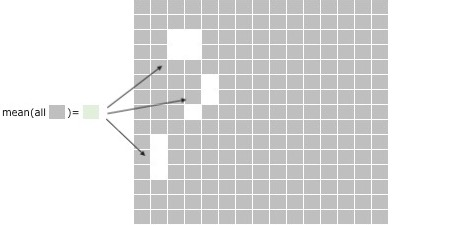
\includegraphics[height=4.1cm]{images/step2.jpg}
         \caption{Compute the mean of the available data (grey squares) and represent it by the green square. This value is then used to substitute the missing data.}
         \label{fig:step2}
     \end{subfigure}
     \hfill
     \vspace{0.5cm}\\
     \begin{subfigure}[b]{0.4\textwidth}
         \centering
         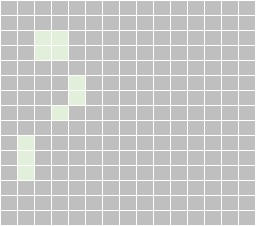
\includegraphics[height=4.1cm]{images/step3.jpg}
         \caption{The resulting sub-dataset for the given site and time after substitution.}
         \label{fig:step3}
     \end{subfigure}
        \caption{Illustration of Grouped Mean Substitution for Handling Missing Data}
        \label{fig:missing_mean}
\end{figure}

 It is important to note that if all 225 grids (15x15) of a time-site pair lack available values from which to calculate the mean, then this entire grid for the time-site pair will remain empty. Such cases might require further action for handling missing data, which will be discussed in the following sections.

\subsection{Negative Value and Zero Substitution}

After implementing the grouped mean substitution, two additional imputation techniques were employed to address any remaining missing points in the dataset: 

\begin{itemize}
    \item \textbf{Missing values were replaced with a negative number, i.e., -10.} This value was chosen because it falls outside the typical range of values in the dataset, ensuring it can be easily identified as a placeholder and not confused with legitimate data.
    \item \textbf{Missing values were substituted with zeros.} The reason for using zero is its neutral nature, which might be less intrusive than other arbitrary values.
\end{itemize}

\section{Predictive Models}
\label{sec:predictive}
This section describes the various models, starting with simple models such as a Baseline model to more complex models like neural
networks (NNs), we used to forecast pollution risk increase or not.

\subsection{Baseline}
We first started with the baseline model, and we used a 5-fold CV on training data to get the baseline of Accuracy, Area under the ROC curve, Precision, Recall, Area under the precision-recall curve and F1-score.

\begin{equation}
\mathrm{Baseline}_k=\sum_{k=1}^5 \frac{1}{5} \mathrm{baseline}_k
\end{equation}

The baseline is the result of random choice. In each fold of validations, the idea is to choose 'predicted Y' randomly from 'training data', and get results with 'true Y' in 'validation data'. The final step is computing the average of the results in each fold. The baseline will serve as a benchmark for all other models.

\subsection{Logistic Regression}
Logistic Regression was chosen as the classification model for this study due to its suitability for binary classification problems and its interpretability. The model estimates the probabilities using a logistic function, providing a probabilistic approach to classifying instances into two distinct classes.

The logistic regression model was fit to the training data using maximum likelihood estimation. The goal is to find the $\beta$ values that maximize the log-likelihood function, which is 
\begin{equation}
\begin{split}
\ell(\beta) & = \log P\left(Y_i=1 \mid \mathbf{X}_i\right) + \log \left(1-P\left(Y_i=1 \mid \mathbf{X}_i\right)\right), \\
\text{where} \quad P(Y=1 \mid \mathbf{X}) & =\frac{1}{1+e^{-\left(\beta_0+\beta_1 X_1+\beta_2 X_2+\ldots+\beta_p X_p\right)}}
\end{split}
\end{equation}
The decision boundary for classification is $P(Y=1 \mid \mathbf{X})=0.5$. If the predicted probability is greater than 0.5, the observation is classified into class 1; otherwise, it is classified into class 0.

\noindent\textbf{Hyperparameter Tuning}

To deal with imbalanced labels in the dataset, Class weight is set to ‘balanced’. It can automatically adjust weights inversely proportional to class frequencies in the input data. SAGA (Stochastic Average Gradient Descent) is selected as the optimization technique because of its efficiency with large datasets.

\begin{itemize}
    \item \verb|penalty|: Regularization types, including Lasso, Ridge, and \verb|elasticnet| (linear combination of Lasso and Ridge).
    \item \verb|C|: Inverse regularization strength parameter, denoted commonly by $\lambda$ in many mathematical formulations. Smaller values of \verb|C| signify stronger regularization, meaning the model will be more penalized for having larger coefficients. It can help to prevent the model being overfitting to the training data.
    \item \verb|l1_ratio|: This hyperparameter is only used when regularization type is \verb|elasticnet|, it represents the ratio of Lasso in the linear combination.
\end{itemize}

\subsection{Random Forest}
Random Forest(RF) is an ensemble learning method that creates multiple decision trees during training and makes a decision by aggregating the results of these individual trees. Each tree gives a classification by training on a random subset of features and samples from the training data. The final decision is based on the mode classification across all trees in the forest which can be represented as:

\begin{equation}
f(x) = \frac{1}{K} \sum^K_{k=1} f_k(x)
\end{equation}
where \( f_k(x) \) is the prediction of the k-th decision tree, and \( K \) is the total number of trees in the forest.

The Random Forest Classifier was also employed due to its effectiveness in handling binary classification problems, its robustness to overfitting, and its ability to handle large datasets with higher dimensionality.

\noindent\textbf{Hyperparameter Tuning}

To optimize performance, various hyperparameters were fine-tuned using a grid search on a validation set. A grid search was conducted over a parameter space consisting of 162 combinations, including 5 critical parameters. This approach was adopted to assess a wide range of parameters while maintaining the computational time at a manageable level.

For consistency and reliability in the search results, certain hyperparameters were kept constant throughout all evaluations. \verb|random_state| was set to a specific value to ensure the reproducibility of results, thus allowing for consistent model production across different runs. \verb|class_weight| was set to 'balanced' due to the imbalance of the 'riskLevelLabel', and \verb|n_jobs| was set to -1 to ensure the use of all available processors and expedite the training process.

The hyperparameters included in the grid search are 
\begin{itemize}
    \item \verb|max_features|: The number of features considered when searching for the best split can affect the speed and performance of the training process. Using \verb|None| means all features are used, while \verb|'sqrt'| means the square root of the total number of features which could help to avoid overfitting.
    \item \verb|max_depth|: The maximum depth of the tree. Using a \verb|None| value means nodes will be expanded until all leaves are pure or until all leaves contain fewer than \verb|min_samples_split| samples. A depth of 10 was also explored to prevent overfitting by limiting the growth of the tree.
    \item \verb|min_samples_split|: The minimum number of samples required to split an internal node. The smallest values of 2 and 5 were tested to control the tree's growth and potentially improve its generalization.
    \item \verb|min_samples_leaf|: The minimum number of samples required to be at a leaf node.  It serves a similar purpose as \verb|min_samples_split|, helping to control the growth of the tree. Values of 1 and 2 were tested in the study.
    \item \verb|n_estimators|: The number of trees in the forest.  Increasing the number of estimators often yields a better-performing model. However, this also results in increased computational demand. 300, 500, and 1000 were the values evaluated. 
\end{itemize}

Models were trained using all 162 combinations of hyperparameters and evaluated using the F1 score to find the best model.

\subsection{Multi-layer Perceptron Classifier}
A Multi-Layer Perceptron (MLP) is a feedforward artificial neural network model that maps sets of input data onto a set of appropriate outputs. It was chosen due to its capability to model complex non-linear relationships.

An MLP consists of three layers of nodes, which are the input layer, hidden layers, and output Layer (see Figure \ref{fig:mlp_architecture}). 

\begin{figure}[H]
\begin{center}
\scalebox{1}[0.9]{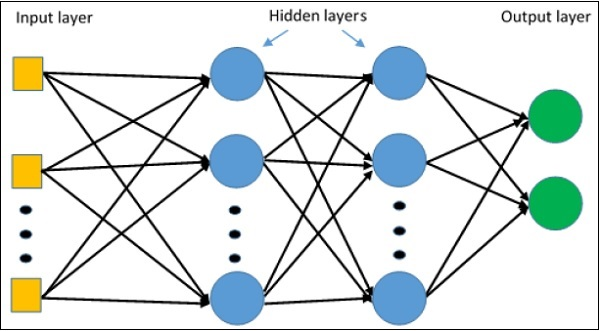
\includegraphics[width=0.8\textwidth]{images/MLP_method.png}}
\caption{MLP Architecture}
\label{fig:mlp_architecture}
\end{center}
\end{figure}
The training process of MLP \citep{485891} involves feedforward propagation and backpropagation, repeated the following steps until convergence: 
\begin{enumerate}
    \item The data is fed into the input layer, and in the hidden layers, each neuron calculates a linear combination of its input, weights, and bias (these values are initialized randomly), $z_i=\sum_j w_{i j} X_j+b_i$; then an activation function (e.g. ReLU, sigmoid, or tanh) is applied to introduce non-linearity, $a_i=f\left(z_i\right)$. This result is passed to the next hidden layers and repeat the process in the same way in the upcoming hidden layers.
    \item  Once the final output is obtained, a loss function calculates how far the predicted output is from the actual target. The loss function is $L(Y, \hat{Y}) = - \left( Y \log(\hat{Y}) + (1 - Y) \log(1 - \hat{Y}) \right)$, where $Y$ is the true label and $\hat{Y}$ is the predicted probability of the class label being 1.
    \item To minimise the loss function, it computes the gradient of the loss function with respect to each parameter by applying the chain rule of calculus from the output layer back to the input layer. Then optimization algorithm (like SGD, Adam, etc.)  is applied on these gradients to update the weights and biases: $w_{ij} = w_{ij} - \alpha \frac{\partial L}{\partial w_{ij}}$ and $b_{i} = b_{i} - \alpha \frac{\partial L}{\partial b_{i}}$.
\end{enumerate}

The decision boundary for classification is $\hat{Y}=0.5$. If the predicted probability is greater than 0.5, the observation is classified into class 1; otherwise, it is classified into class 0.

\noindent\textbf{Hyperparameter Tuning}

To deal with imbalanced labels in the dataset, oversampling was applied on the minority label. 

\begin{itemize}
    \item \verb|hidden_layer_sizes|: A tuple where the length is the number of hidden layers and each element represents the number of neurons in that layer.
    \item \verb|activation|: The activation function for the hidden layers, including Rectified Linear Activation, Hyperbolic tangent function, and Logistic sigmoid function. 
    \item \verb|solver|: The algorithm for weight optimization, including Adaptive momentum, Stochastic Gradient Descent and Limited-memory BFGS.
    \item \verb|learning_rate|: The step size at each iteration while moving towards a minimum in the loss function, including \verb|'constant'|,\verb|'invscaling'| and \verb|'adaptive'|.
    \item \verb|alpha|: L2 Regularization parameter to prevent overfitting.
\end{itemize}

\subsection{Convolution Neural Network}
A convolution neural network (CNN) allows the spatial relation between points to be taken into consideration, unlike all our other models, which take the engineered features as inputs. Comparisons between CNN and our other models would give insight into whether the spatial relation between points is important, and whether deriving more sophisticated features based on these spatial relations could improve the signals extracted. 

CNNs are deep-learning algorithms that take an image as input and assign importance to aspects or objects within the image, usually for the end result of classifying images. It has a similar basic structure as the MLP model applied to engineered features, with an input layer, hidden layers, and an output layer, and is trained in a similar manner as an MLP with backpropagation to minimise a loss function. The difference between a CNN and an MLP model lies in its hidden layers. While the hidden layers of an MLP model are all fully-connected layers, a CNN has hidden convolution layers and pooling layers on top of fully-connected layers. Convolution layers use kernels that 'slide' over the input data, where every time a kernel stops, an elementwise multiplication is performed between the kernel and the input layer, with the result being a part of the next layer, and ultimately with many kernel stops combines to generate feature map. When there is more than one kernel or when the input data is not two-dimensional, the resulting output layer could also be of a higher dimension. Convolution layers aim to summarise and generalise features in an image better by sweeping over the image in a similar manner as humans would look at an image. Pooling layers are primarily used to reduce the dimensions of the feature maps by simply summarising the features present in the region of a feature map. While this also involves sliding a kernel across the input data, the kernel simply applies a simple function such as averaging or taking the maximum value of data covered by the kernel, whereas the kernel in a convolution layer has weights to be learned through training. 

To apply CNN to our dataset, the feature values were arranged spatially and treated as pixel values, with the values for different features stacked together and acting as different channels to create a 15 x 15 x 6 tensor for every time-site pair. This is reminiscent of how in coloured images, each pixel can be represented by a combination of a few key colours, and thus the colours act as different channels, and the channels are stacked together to create an input into the neural network. 

\textbf{Neural Network Architecture.} The CNN architecture applied is based on the LeNet architecture, which is a relatively simple convolutional neural network structure proposed in 1998 to identify handwritten digits \citep{lecun1998gradient}. Though the model is relatively simple, it was found to exhibit good performance on the MNIST dataset, which was trained on 60,000 black and white images with a dimension of 28 x 28. As the MNIST dataset is somewhat similar in scale to our data, with a training dataset of 112,266 15 x 15 x 6 tensors, it seems that the architecture is suited for our dataset. Experiments on fundamentally altering the architecture of LeNet did not yield significantly improved results. However, several changes were made to shape the model for our use case and improve the overall performance of the model, with some techniques stemming from research published long after LeNet was first introduced. 

\begin{enumerate}
    \item An additional fully-connected layer was added as the final layer such that it became the output layer, where the layer had one node and a Sigmoid activation function. This allows the final output to be a single probability between 0 and 1 to achieve our purpose of binary classification.
    \item Filter size and padding were adjusted to fit our image of a lower resolution. As our input image has an odd number resolution of 15x15 as compared to 32x32 in the MNIST dataset, padding was added before the first pooling layer to ensure no data loss. Furthermore, as our dataset started with a smaller input image, the kernel in the second layer was reduced to 3x3 to ensure the output after the final max-pooling layer is not just a 1x1 point. 
    \item  Regularisation techniques were employed to prevent overfitting of the neural network model, namely weight decay and dropout, which is especially important given the high level of noise in our dataset. Weight decay ($L_2$ regularisation) was applied to the weights in both the convolutional and fully-connected layers to penalise a larger weight value and encourage smaller weights. Formulaically, this changes the calculated loss as shown below, with $w$ representing weights:
    \begin{equation}
    L_{new} = L_{original}(w) + \lambda w^T w 
    \end{equation}
    The lambda chosen for the convolution layer was chosen to be 0.0005, as this value was used in several landmark CNN papers \citep{krizhevsky2012imagenet} \citep{simonyan2014very}, where \citep{krizhevsky2012imagenet} also reported that weight decay not only acted as a regulariser but also helped the model learn. Lambda for the fully connected layers was chosen as 0.01 as it was a common default value used. Dropout was added in between each fully connected layer, where at each layer a certain percentage of nodes would be randomly ignored during training \citep{srivastava2014dropout}. The dropout percentage, which refers to the probability that a node in a fully connected layer was dropped out in the training stage, is a tuning parameter of the model. A non-zero dropout probability helps prevent overfitting, but having too high of a dropout probability could impede the model's ability to learn. 
    \item Batch normalisation was added in each convolution layer to speed up and stabilise training of the model \citep{ioffe2015batch}. This re-centres and re-scales each batch of input data before feeding it into the network. It was added before ReLU activation for each layer as described in the original batch normalisation paper.
    \item Pooling layers used max-pooling instead of average pooling. Though both average and max pooling is commonly used, there is some research that suggests max pooling outperforms average pooling as it leads to faster convergence and improves generalisation \citep{boureau2010theoretical, scherer2010evaluation}. Furthermore, intuitively max pooling is better at identifying sharp features than average pooling, which seems likely to improve model performance for noisier datasets such as ours.
    
\end{enumerate}
Figure \ref{fig:cnn_architecture} illustrates the architecture of the neural network used. 

\begin{figure}[H]
\begin{center}
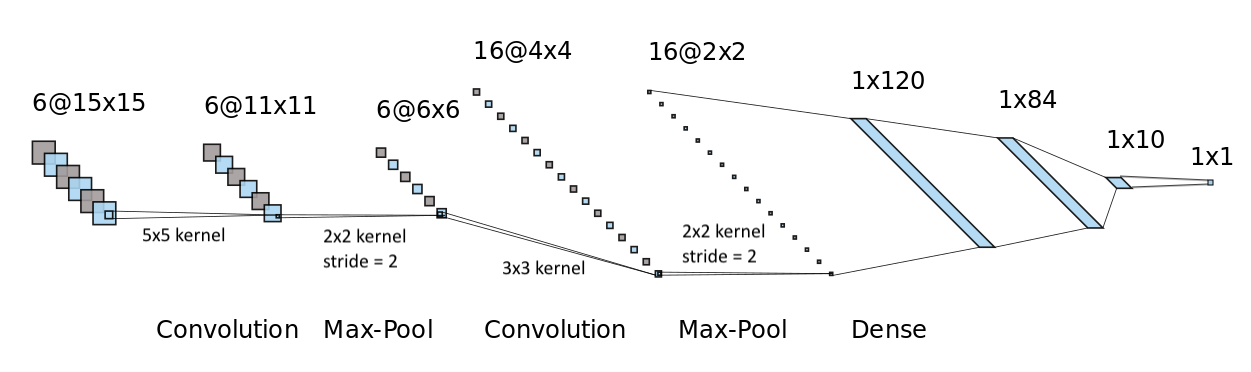
\includegraphics[width=\textwidth]{images/cnn_architecture.png}
\caption{CNN Architecture}
\label{fig:cnn_architecture}
\end{center}
\end{figure}

\textbf{Loss Function.} The loss function to be minimised for our CNN is a weighted binary cross-entropy loss. $w_1$ represents how many more times the weight given to the minority class is, compared to the majority class. $Y_i$ is the true label and $\hat{Y_i}$ is the predicted probability of the class label being 1 for a particular data point i, with $Y$ and $\hat{Y}$ being a vector representation of $Y_i$ and $\hat{Y_i}$.

\begin{equation} 
\label{eqn:weighted_bce_loss}
L(Y, \hat{Y}) = - \frac{1}{N} \sum^{N}_{i=1} [Y_i \cdot log \hat{Y_i} \cdot w_1 + (1-Y_i) \cdot log (1-\hat{Y_i})]
\end{equation}
If $w_1 = 1$ the loss function becomes the standard binary cross entropy-loss; more weight is given to the minority class when $w_1 > 1$. $w_1$ is a tuning parameter for the model. It was found that our model performance is highly sensitive to the weight - if $w_1$ is too small, all the predictions in the model become 0, while if $w_1$ is too big, all the predictions become 1.

\textbf{Optimiser} 
The model uses an Adam optimiser as proposed in \citep{kingma2014adam}. The learning rate of the model is a hyperparameter to be tuned in the model to ensure that the model does not train too slowly while also does not encounter exploding gradient issues.

\textbf{Data Augmentation.}
To tackle the highly imbalanced dataset, 'oversampling' was performed on the minority class through data augmentation. Literature has shown that neural networks are not well suited for training imbalanced data \citep{raj2016towards}, and thus by performing data augmentation it is hoped that the dataset can be made less unbalanced while 'images' passed into the model would not strictly be repeated. Data augmentation was done for each sample in the minority class on the training dataset by flipping the image horizontally and vertically, then for each of the original images, horizontally flipped image and vertically flipped image, rotate the image by 90, 180 and 270 degrees. This increases the number of positive samples twelve-fold. 

\textbf{Batch Size and Epochs.} The batch size was fixed to be 64 heuristically, as it should not greatly impact the f1 score. Training epochs were set to 500 as an upper limit, though it is unlikely any setting would lead to the model training for 500 epochs due to the presence of the patience parameter. 

\textbf{Decision Boundary.} Similar to MLP and LR, the decision boundary for classification is $\hat{Y} = 0.5$. If the predicted probability is greater
than 0.5, the observation is classified into class 1; otherwise, it is classified into class 0

\textbf{Hyperparameter Tuning.} Hyperparameter tuning was performed on both datasets where we filled missing values with 0 and filled missing values with -10 to arrive at a near-best CNN model with both datasets. It was performed iteratively until we saw minimal further improvements in the f1 score. It was found that the model was quite sensitive to a few hyperparameters in particular, such that altering these hyperparameters slightly could lead to the model either giving predictions of all 0 or 1. In summary, the hyperparameters and the values trialled are: 

\begin{enumerate}
    \item Adam learning rate. Learning rates between 0.000001 and 0.0001 were explored. 
    \item Dropout probability. We trialled values from 0 to 0.2. Note that the dropout probability is fixed for all the fully connected layers. 
    \item Loss weight. This is denoted by $w_1$ in the loss equation in equation \ref{eqn:weighted_bce_loss}. Based on some initial experimentations, we tuned the hyperparameter with values from 2 to 5. 
    \item Patience. This stems from using early stopping to stop training the neural network models hopefully before they overfit. Patience refers to the number of epochs to wait before stopping where we see no improvement in the validation f1 score. Values between 10 and 50 were trialled. 
\end{enumerate}

\section{Principle Component Analysis for Dimension Reduction}

Before trying PCA (Principle Component Analysis) \citep{bro2014principal}, we tried forward selection with Logistic Regression. However, it was too computationally expensive, and our dataset is large, so it was not a practical method for dimension reduction. PCA could be much more efficient. From Figure \ref{fig:PCA}, it can be seen that more than 99\% of variance could be explained with just 5 components.

\begin{figure}[H]
\begin{center}
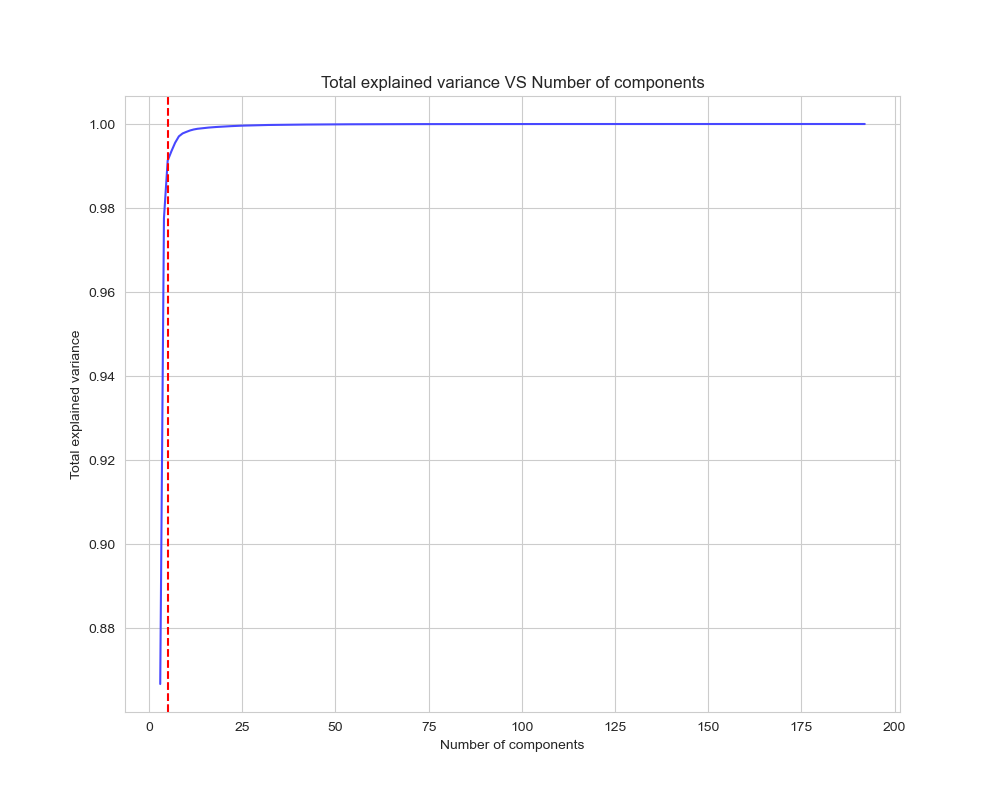
\includegraphics[height=0.5\textwidth]{images/PCA_for_mean.png}
\caption{Explained Variance vs Number of components}
\label{fig:PCA}
\end{center}
\end{figure}

\begin{table}[H]
    \centering
    \caption{Results with PCA vs results without PCA}
    \label{table:PCA_comparion}
    \begin{tabular}{
        l
        S[table-format=1.3]
        S[table-format=1.3]
        S[table-format=1.3]
        S[table-format=1.3]
        S[table-format=1.3]
    }
    \toprule
    \textbf{Model} & {\textbf{F1}} & {\textbf{Precision}} & {\textbf{Recall}}  & {\textbf{AP}} & {\textbf{ROC-AUC}} \\
    \midrule
    LR with PCA & 0.073 & 0.039 & 0.610 & 0.034 & 0.597 \\
    \addlinespace
    LR without PCA & 0.073 & 0.039 & 0.610 & 0.034 & 0.597 \\
    \addlinespace\midrule
    MLP with PCA & 0.074 & 0.040 & 0.663 & 0.035 & 0.610 \\
    \addlinespace
    MLP without PCA & 0.076 & 0.040 & 0.610 & 0.037 & 0.625 \\
    \bottomrule
    \end{tabular}
\end{table}

It can be seen from Table \ref{table:PCA_comparion} that LR and MLP could get similar results with or without PCA. Although the performance of MLP with PCA is slightly worse than that without PCA,  it saved lots of time for hyperparameter tuning process. The results for LR with PCA did not decrease, and the time for hyperparameter tuning for LR was just within 2 minutes.



\chapter{Numerical Experiments}

This section presents the results of applying various binary classifiers to the S3 data for predicting sewage pollution, while also highlighting and addressing numerous lines of inquiry that were raised as we explored the datasets and models. Firstly, hyperparameter tuning was done to arrive at the best version of each model outlined in the methodology section \label{sec:predictive} with our main S3 datasets. Secondly, we dived deeper into investigating where each of the best models made the best and worst predictions. Thirdly, we explored the gains from creating engineered features by comparing models trained on raw data and models trained on engineered features specifically. Fourthly, we did a comparison between running models on S2 and S3 data, providing insights into the tradeoff between spatial resolution and temporal frequency. Finally, models on varying window sizes were retrained to find at what point increasing window size no longer yields positive improvements to model performance. The models were run primarily on our local laptops, with some models running on Google Colaboratory in a high RAM environment for when local computation resources were insufficient, such as with the convolutional neural network on S2 data.

\begin{comment}
\section{Comparison of Best Models (OLD SECTION, TO BE DELETED)}

\qs{rephrase and elaborate} Firstly, hyperparameter tuning was done to arrive at the best version of each model outlined in the methodology section with our main S3 datasets.


\subsection{Logistic Regression}


\paragraph{Sentinel 3 (Fill Nan with 0)}
The best hyperparameters on this dataset is \verb|{'penalty': 'elasticnet', 'C': 0.01, 'l1_ratio': 0.25}|, which means 25\% of Lasso and 75\% of Ridge, $\lambda$ = 0.01
\paragraph{Sentinel 3 (Fill Nan with -10)}
In this dataset, logistic regression had difficulty to converge during the process of hyperparameter tuning. For the other one, the model can converge with 5000 iterations. But for this one, the model with several combinations of hyperparameter still not converge even the maximum number of iterations increased to 20,000. One possible reason might be logistic regression became less sensitive when the values of X are more top-heavy, since the missing values are filled with -10, then \verb|MinMaxScaler| (\( X_{\text{scaled}} = \frac{X_{\text{max}} - X_{\text{min}}}{X - X_{\text{min}}} \)) is applied on the dataset. If keep increasing the maximum number of iterations, the tuning process will be computationally expensive and time-consuming. Due to these reasons, logistic regression might not had found the 'best' combination of hyperparameters on this data.

\qs{\subsubsection{Forward Selection using Logistic Regression}
We applied forward selection by trying every available feature to fit the training data, and see which had the best performance on validation data, iterating this process until there was no progress. Due to the size of the datasets, this method is computationally expensive. We discarded this method.}



\subsection{Random Forest}

After conducting the grid search over the specified parameter space, the results were evaluated using the f1 score for both datasets. The search identified the optimal hyperparameters for both datasets shown in \ref{table:rf_best_hyperparamters}.

Given that the hyperparameter tuning did not significantly improve the f1 score and to prevent unnecessary computational costs, a decision was made not to explore a broader parameter space. The exploration will proceed using the best parameter combinations found.

\begin{table}[h]
        \caption{RF Best Hyperparameters}
        \label{table:rf_best_hyperparamters}
        \centering
        \begin{tabular}{lccccc}
        \toprule
         & \verb|max_features| & \verb|max_depth| & \verb|min_samples_split| & \verb|min_samples_leaf| & \verb|n_estimators| \\
        \midrule
        S3 F0 & log2 & 10 & 5 & 1 & 1000 \\
        S3 F-10 & log2 & 10 & 5 & 1 & 1000 \\ \bottomrule
        \end{tabular}
\end{table}

\subsubsection{Model Performance}

\begin{figure}[h]
    \centering
    \begin{subfigure}[b]{0.45\textwidth}
        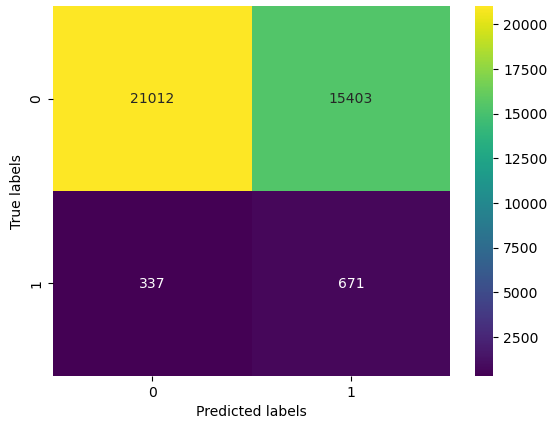
\includegraphics[width=\textwidth]{images/cm_rf.png}
        \caption{Confusion Matrix for RF}
        \label{fig:cm_rf}
    \end{subfigure}
    \hfill
    \begin{subfigure}[b]{0.45\textwidth}
        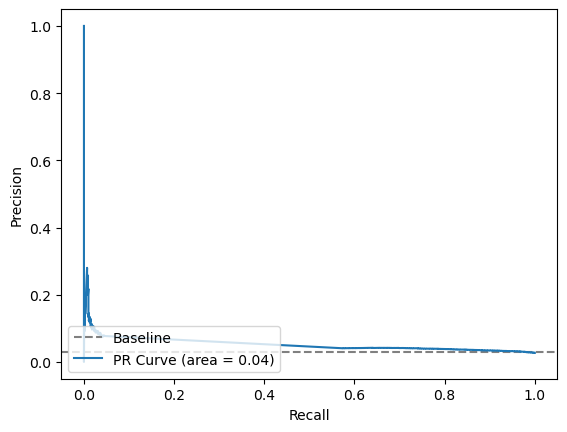
\includegraphics[width=\textwidth]{images/pr_rf.png}
        \caption{Precision-Recall Curve for RF}
        \label{fig:prc_rf}
    \end{subfigure}
    \hfill
    \begin{subfigure}[b]{0.45\textwidth}
        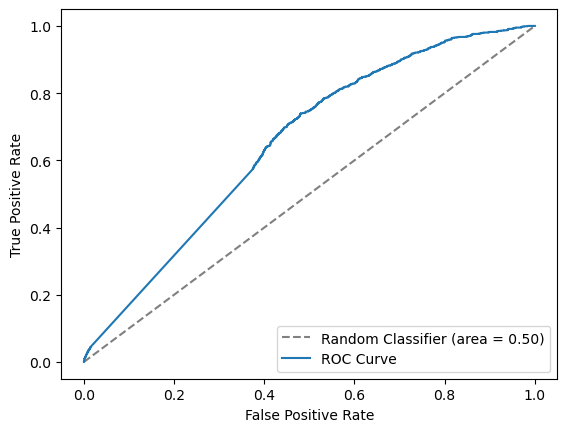
\includegraphics[width=\textwidth]{images/roc_rf.png}
        \caption{ROC Curve for RF}
        \label{fig:roc_rf}
    \end{subfigure}
    \caption{Performance for RF on S3 (Fill Nan with 0)}
\end{figure}

\subsection{Multi-layer Perceptron Classifier}

After hyperparameter tuning, results showed that the MLP model had the best optimiser on Sentinel 3 (Fill Nan with 0) is 'Adam', and the best optimiser on Sentinel 3 (Fill Nan with -10) is 'SGD'.

\end{comment}

\section{Comparison of Best Models}
\label{sec:Comparison of Best Models}

\subsection{Hyperparameter Tuning}

An iterative grid search was executed across the designated parameter spaces for each model, and the performance was assessed using the F1 score. This approach selected the optimal hyperparameters for all models on both datasets; the final selection of hyperparameters for each model is detailed in table  \ref{tab:best_hyper}.

The chosen hyperparameters for each model appear remarkably similar for both datasets S3 F0 and S3 F-10. They are identical for RF and CNN, while only one parameter differs for RF and MLP. One potential reason for this consistency could be the similarity in the distribution of datasets when using 0 or -10 as the placeholder for missing data. Another possible reason is the iteration of hyperparameter combinations for CNN is interrupted when the score gradually stabilizes. For other models, hyperparameter combinations were only tested within the predefined parameter spaces. As a result, not all possible combinations were explored, and the outcome might be influenced by the selection of these parameter spaces.

\begin{table}[H]
    \centering
    \caption{Best Hyperparameters}
    \begin{subtable}{\linewidth}
        \centering
        \caption{LR Best Hyperparameters}
        \label{table:lr_best_hyperparamters}
        \begin{tabular}{lccccc}
        \toprule
        \textbf{Data} & \verb|penalty| & \verb|C| & \verb|l1_ratio|  \\
        \midrule
        S3 F0 & 'elasticnet' & 0.01 & 0.25 \\
        S3 F-10 & 'elasticnet' & 0.01 & 0.1 \\ \bottomrule
        \end{tabular}
    \end{subtable}
    \bigskip
    
    \begin{subtable}{1.1\linewidth}
        \centering
        \caption{RF Best Hyperparameters}
        \label{table:rf_best_hyperparamters}
        \begin{tabular}{lccccc}
        \toprule
        \textbf{Data} & \verb|max_features| & \verb|max_depth| & \verb|min_samples_split| & \verb|min_samples_leaf| & \verb|n_estimators| \\
        \midrule
        S3 F0 & log2 & 10 & 5 & 1 & 1000 \\
        S3 F-10 & log2 & 10 & 5 & 1 & 1000 \\ \bottomrule
        \end{tabular}
    \end{subtable}
    \bigskip
    
    \begin{subtable}{\linewidth}
        \centering
        \caption{MLP Best Hyperparameters}
        \label{table:mlp_best_hyperparamters}
        \begin{tabular}{lccccc}
        \toprule
        \textbf{Data} & \verb|hidden_layer_sizes| & \verb|activation| & 
            \verb|learning_rate| & \verb|alpha| & \verb|solver|  \\
        \midrule
        S3 F0 & (400, 800, 400, 200) & 'relu' & 'adaptive' & 0.0001 & 'adam' \\
        S3 F-10 & (400, 800, 400, 200) & 'relu' & 'adaptive' & 0.0001 & 'sgd' \\ \bottomrule
        \end{tabular}
    \end{subtable}
    \bigskip
    
    \begin{subtable}{\linewidth}
        \centering
        \caption{CNN Best Hyperparameters}
        \label{tab:cnn_best_hyperparamters}
        \begin{tabular}{lcccc}
        \toprule
        \textbf{Data} & \verb|adam_learning_rate| & \verb|dropout| & \verb|loss_weight| & \verb|patience| \\
        \midrule
        S3 F0 & 0.00005 & 0.075 & 3 & 30  \\
        S3 F-10 & 0.00005 & 0.075 & 3 & 30  \\ \bottomrule
        \end{tabular}
    \end{subtable}
    \label{tab:best_hyper}
\end{table}
    
\subsection{Summary of Results}


Table \ref{tab:all_hyperparameter_results} presents the performance of all the models of interest. These models were trained and tuned using the same groups of time-site pair for the training and validation sets of the S3 F0 and S3 F-10 datasets, which were subsequently tested on the test set of the S3 dataset. The metrics used for comparison include F1-score, Precision, Recall, AP, and ROC-AUC.

\begin{table}[h]
    \caption{Model Performance Comparison Using Best Hyperparameters on S3 Data}
    \label{tab:all_hyperparameter_results}
    \centering
    \begin{tabular}{lccccccc}
    \toprule
    \textbf{Model} & \textbf{Data} & \textbf{F1} & \textbf{Precision} & \textbf{Recall} & \textbf{AP} & \textbf{ROC-AUC}  \\
    \midrule
    Baseline & S3 & 0.024 & 0.024 & 0.025 & 0.027 & 0.498 \\ \midrule
    LR & S3 F0 & 0.073 & 0.039 & 0.610 & 0.034 & 0.597  \\
     & S3 F-10 & 0.075 & 0.040 & 0.619 & 0.034 & 0.603 \\ \midrule
    RF & S3 F0 & \textbf{0.079} & \textbf{0.042} & 0.666 & \textbf{0.043} & \textbf{0.651}    \\
     & S3 F-10 & \textbf{0.079} & \textbf{0.042} & 0.666 & \textbf{0.043} & \textbf{0.651}   \\ \midrule
    MLP & S3 F0 & 0.076 & 0.040 & 0.620 & 0.035 & 0.607  \\
     & S3 F-10 & 0.076 & 0.040 & \textbf{0.735} & 0.037 & 0.625   \\ \midrule
    CNN & S3 F0 & 0.074 & 0.039 & 0.672 & 0.039 & 0.623   \\
     & S3 F-10 & 0.077 & 0.041 & 0.668 & 0.040 & 0.627   \\ \bottomrule
    \end{tabular}
\end{table}

In general, the performance metrics for these models are quite comparable. However, the RF model is particularly notable, consistently emerging as a top performer across most metrics. Additionally, all models significantly outperform the baseline, which has notably low scores in all metrics, highlighting the importance of model selection for achieving optimal performance.

The performance of all models using the S3 F-10 dataset is generally better than those using S3 F0, as indicated by the investigated metrics. For models like the MLP, the disparities are more pronounced, especially for recall, while the performances of both datasets on RF are completely the same. This suggests that using -10 as a placeholder for missing values in the dataset might be a better choice than 0. Thus, for easier comparison, only the models trained using S3 F-10 are used for all methods except for LR. The result for LR using S3 F-10 did not converge, so subsequent sections continued to use S3 F0 to achieve more stable results.

Regarding the primary metric, the F1 score, RF achieves the highest value, 0.079, for both the S3 F0 and S3 F-10 datasets, which reflect a better balance between Precision and Recall than other models. Most models, including LR, MLP, and CNN, obtained a value around the mid-0.07s, suggesting that the overall quality of predictions is fairly consistent across models.

For precision and recall metrics, the RF model stands out with a precision of 0.042. The CNN, MLP, and LR models closely follow, with precision values around 0.04. MLP on the S3 F-10 data obtained the highest recall at 0.735, indicating it captures a substantial portion of the positive instances. This is further supported by the confusion matrix detailed in figure \ref{fig:cm}, which aligns with the precision and recall findings.

\begin{figure}[h]
    \centering
    \begin{subfigure}[b]{0.52\textwidth}
        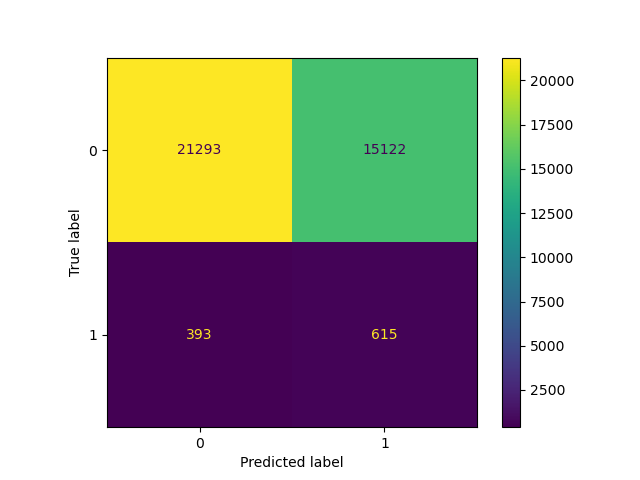
\includegraphics[width=\textwidth]{images/LG_S3_zero_CM.png}
        \caption{Logistic Regression}
        \label{fig:cm_lr}
    \end{subfigure}
    \hfill
    \begin{subfigure}[b]{0.44\textwidth}
        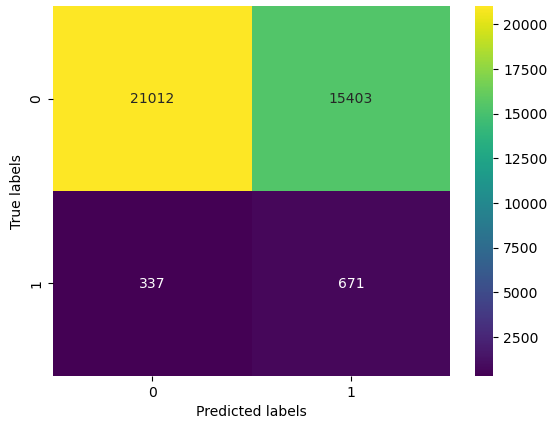
\includegraphics[width=\textwidth]{images/cm_rf.png}
        \caption{Random Forest}
        \label{fig:cm_rf}
    \end{subfigure}
    \hfill
    \begin{subfigure}[b]{0.52\textwidth}
        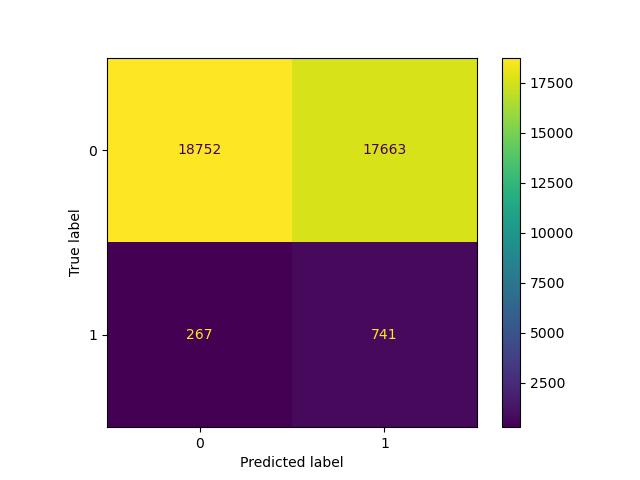
\includegraphics[width=\textwidth]{images/MLP_S3_neg_CM.png}
        \caption{Multi-Layer Perceptron}
        \label{fig:cm_mlp}
    \end{subfigure}
    \hfill
    \begin{subfigure}[b]{0.43\textwidth}
        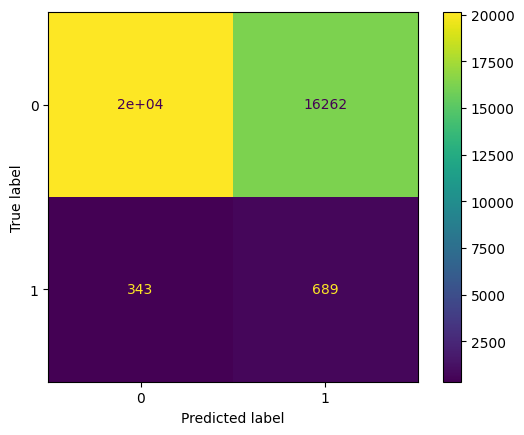
\includegraphics[width=\textwidth]{images/cm_cnn_neg10.png}
        \caption{Convolutional Neural Network}
        \label{fig:cm_cnn}
    \end{subfigure}
    \caption{Confusion Matrices for Best Models}
    \label{fig:cm}
\end{figure}

All models exhibit limited capabilities to differentiate between classes, as reflected by their ROC-AUC scores and the curves displayed in \ref{fig:roc_pr}. The RF model remains the highest, with a score of 0.651. Other models, such as the MLP and CNN, have ROC-AUC values in the 0.6s range, highlighting their constrained discrimination abilities.

\begin{figure}[H]
\centering
\begin{subfigure}[b]{0.45\textwidth} % Adjusted to 0.45 to leave some space between figures
    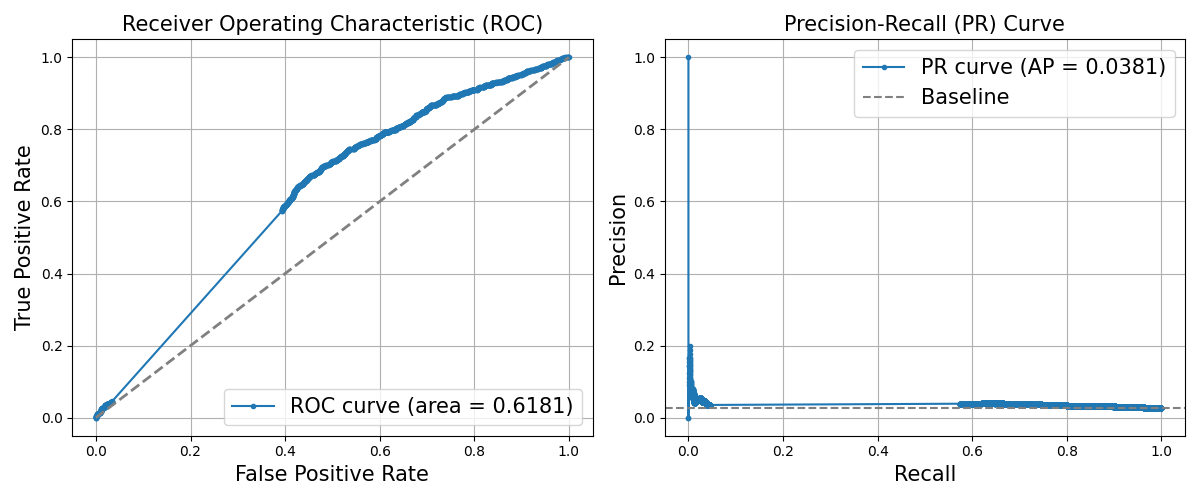
\includegraphics[width=\textwidth]{images/LG_S3_zero_Curves.png}
    \caption{Logistic Regression}
    \label{fig:roc_pr_lr}
\end{subfigure}
\hfill
\begin{subfigure}[b]{0.45\textwidth} % Adjusted to 0.45 to leave some space between figures
    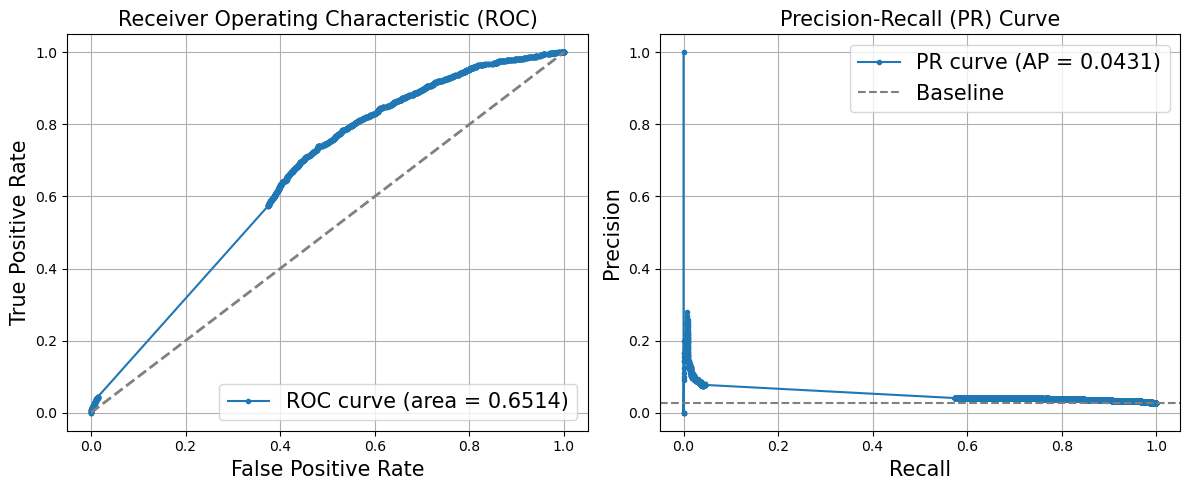
\includegraphics[width=\textwidth]{images/roc_pr_rf.png}
    \caption{Random Forest}
    \label{fig:roc_pr_rf}
\end{subfigure}
\\ % New line here
\begin{subfigure}[b]{0.45\textwidth} % Adjusted to 0.45 to leave some space between figures
    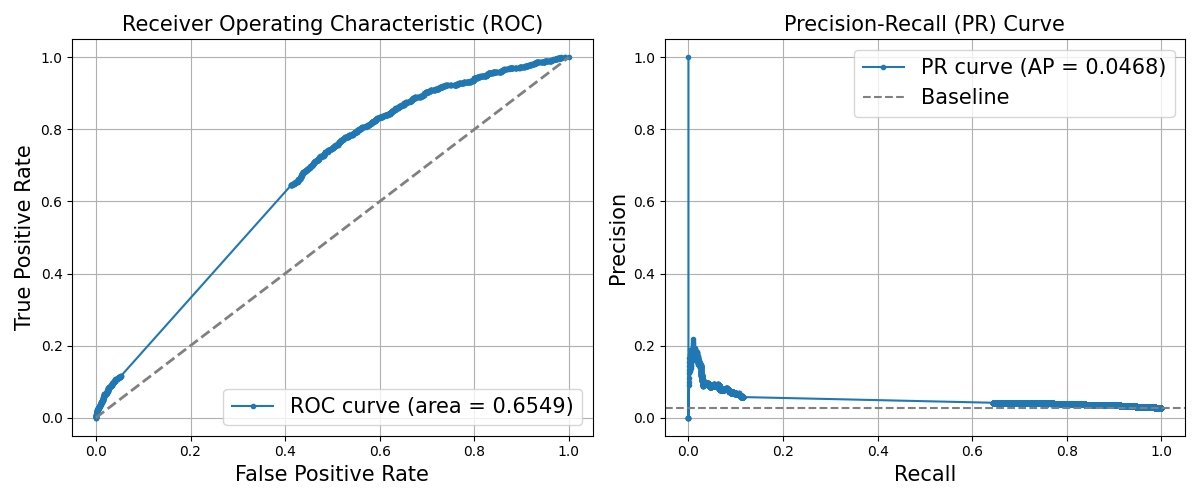
\includegraphics[width=\textwidth]{images/MLP_S3_neg_Curves.png}
    \caption{Multi-Layer Perceptron}
    \label{fig:roc_pr_mlp}
\end{subfigure}
\hfill
\begin{subfigure}[b]{0.45\textwidth} % Adjusted to 0.45 to leave some space between figures
    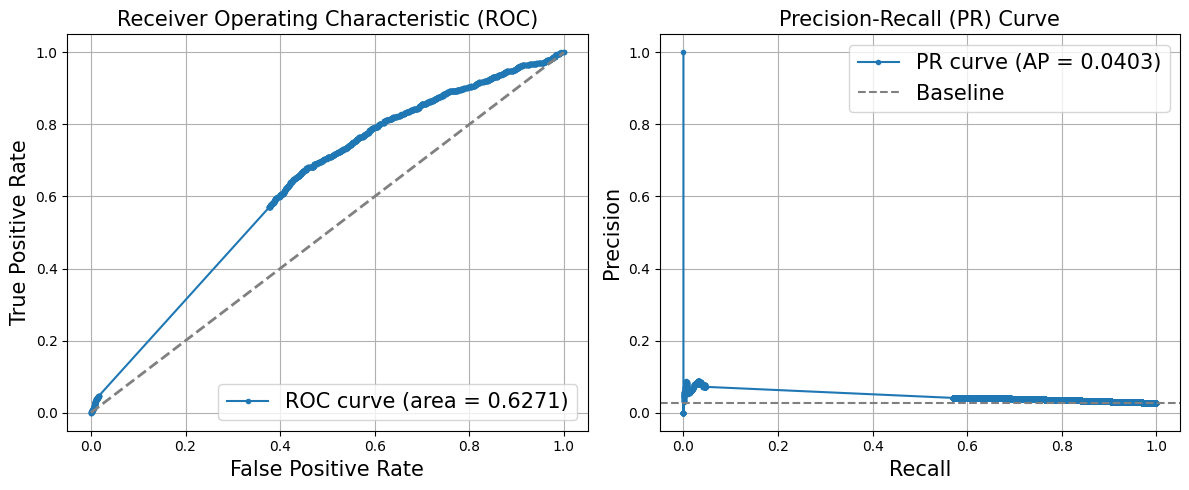
\includegraphics[width=\textwidth]{images/roc_pr_graph_cnn_neg10.png}
    \caption{Convolutional Neural Network}
    \label{fig:roc_pr_cnn}
\end{subfigure}
\caption{ROC and Precision-Recall Curves for Best Models}
\label{fig:roc_pr}
\end{figure}


\section{Strengths and Weaknesses of Best Models}
\label{sec:Strengths and Weaknesses of Best Models}

This section investigates the strengths and weaknesses of the best models found in section 4.1. This was achieved by slicing test predictions by various characteristics, such as years, months and regions, enabling comparisons of model performance across categories. 

Tables \ref{tab:metrics_across_years}, \ref{tab:metrics_across_months}, and \ref{tab:metrics_across_regions} depict the F1 scores of each best model on the test dataset separated by years, months and regions respectively. It also includes figures to help us understand the differences we see, namely the number of data points in each category, the percentage of positive labels that fall under the category in the training dataset, and the percentage of positive labels that fall under the category in the test dataset. 

\subsection{Across Years, Months, Regions}
    \begin{table}[H]
        \caption{F1 Score By Classifier and Year on Test Data. Each classifier is the best for their model class as trained on S3 15x15 windowed data.}
        \label{tab:metrics_across_years}
        \centering
        \begin{tabular}{lccccccc}
        \toprule
        \textbf{Year} & \textbf{Count} & \textbf{\%Pos-Train} & \textbf{\%Pos-Test} & \textbf{LR} & \textbf{RF} & \textbf{MLP} & \textbf{CNN} \\
        \midrule
        2020 & 11766 & \textbf{3.29} & 3.09 & \textbf{0.078} & \textbf{0.086} & \textbf{0.084} & \textbf{0.087} \\
        2021 & \textbf{12894} & 3.08 & \textbf{3.12} & \textbf{0.078} & 0.084 & 0.081 & 0.079  \\ 
        2022 & 12763 & \textbf{3.29} & 2.09 & 0.062 & 0.064 & 0.063 & 0.063 \\ \bottomrule
        \end{tabular}
    \end{table}

    \begin{figure}[H]
        \begin{center}
        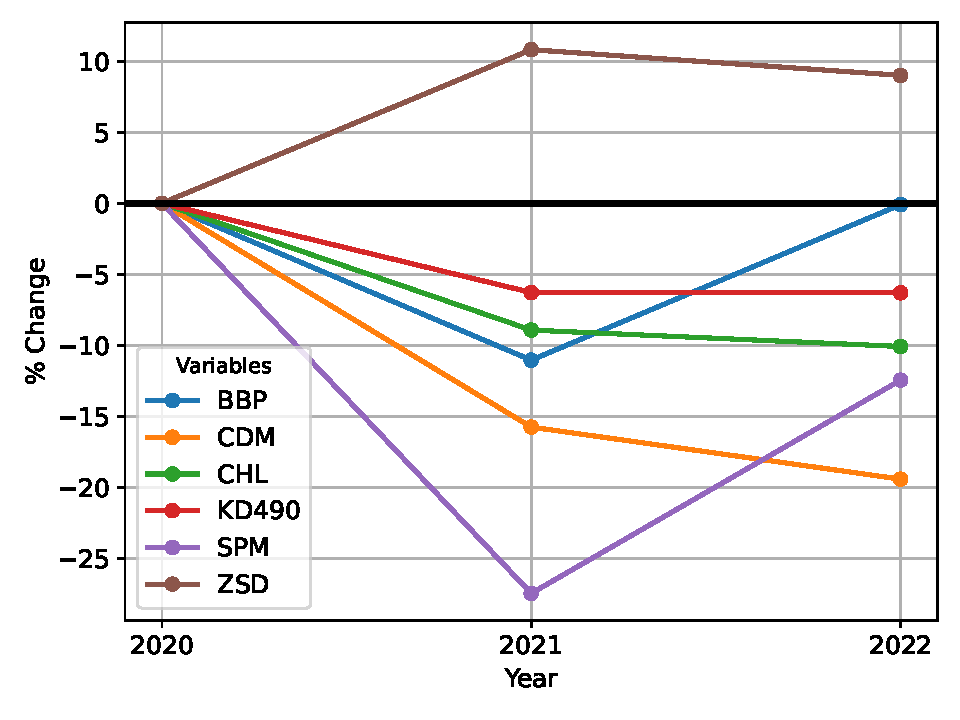
\includegraphics[height=0.2\textheight]{images/percent_change_by_year.pdf}
        \caption{Percentage change in BBP, CDM, CHL, KD490, SPM, ZSD mean values for S3 data at 15x15 window across 2020, 2021 and 2022, with 2020 acting as a base year. The values come from our complete engineered feature dataset for S3 (train and test).}
        \label{fig:pc_by_year}
        \end{center}
    \end{figure}
    

    \begin{table}[H]
        \caption{F1 Score By Classifier and Month on Test Data. Each classifier is the best for their model class as trained on S3 15x15 windowed data.}
        \label{tab:metrics_across_months}
        \centering
        \begin{tabular}{lccccccc}
        \toprule
        \textbf{Month} & \textbf{Count} & \textbf{\%Pos-Train} & \textbf{\%Pos-Test} & \textbf{LR} & \textbf{RF} & \textbf{MLP} & \textbf{CNN} \\
        \midrule
        May & 6430 & 1.56 & 1.54 & 0.045 & 0.053 & 0.053 & 0.053 \\
        June & 7690 & 2.26 & 2.07 & 0.057 & 0.058 & 0.057 & 0.059  \\ 
        July & \textbf{7829} & 1.88 & 1.98 & 0.059 & 0.062 & 0.056 & 0.055 \\ 
        August & 7683 & 3.39 & 3.41 & 0.090 & 0.095& 0.092 & 0.095 \\
        September & 7429 & \textbf{4.62} & \textbf{4.51} & \textbf{0.108} & \textbf{0.114} & \textbf{0.113} & \textbf{0.113} \\\bottomrule
        \end{tabular}
    \end{table}


\begin{figure}[H]
    
        \centering
        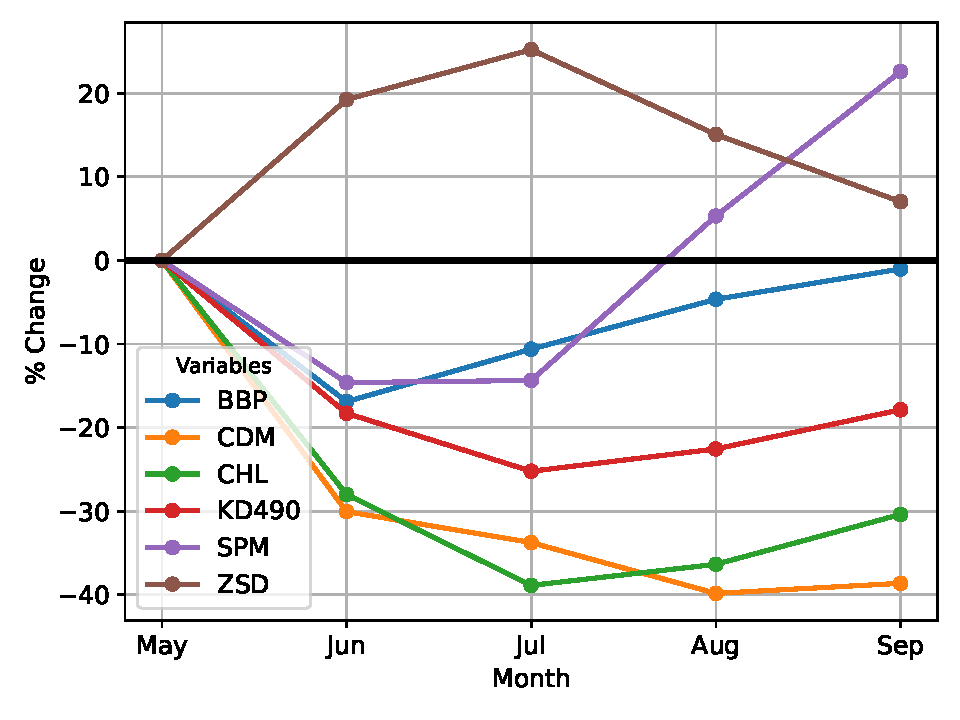
\includegraphics[height=0.2\textheight]{images/percent_change_by_month.pdf}
        \caption{Percentage change in BBP, CDM, CHL, KD490, SPM, ZSD mean values for S3 data at 15x15 window across May, June, July, August and September, with May acting as a base month. The values come from our complete engineered feature dataset for S3 (train and test).}
        \label{fig:pc_by_month}
\end{figure}






    \begin{table}[H]
        \caption{F1 Score By Classifier and Region on Test Data. Each classifier is the best for their model class as trained on S3 15x15 windowed data.}
        \label{tab:metrics_across_regions}
        \centering
        \begin{tabular}{lccccccc}
        \toprule
        \textbf{Regions} & \textbf{Count} & \textbf{\%Pos-Train} & \textbf{\%Pos-Test} & \textbf{LR} & \textbf{RF} & \textbf{MLP} & \textbf{CNN} \\
        \midrule
        South West & 17926 & 2.46 & 2.47 & 0.069 & 0.074 & 0.075 & 0.071 \\
        South East & 7603 & 2.56 & 2.59 & 0.082 & 0.082 & 0.073 & 0.080  \\ 
        East of England & 3510 & 2.15 & 1.85 & 0.034 & 0.043 & 0.045 & 0.044 \\ 
        North East & 2953 & 2.92 & 3.12 & 0.098 & 0.102 & 0.096 & 0.101 \\
        North West & 2557 & \textbf{5.66} & \textbf{5.12} & \textbf{0.110} & \textbf{0.120} & \textbf{0.119} & \textbf{0.120} \\
        Yorkshire & 1832 & 4.21 & 3.82 & 0.081 & 0.082 & 0.076 & 0.074 \\
        East Midlands & 696 & 1.98 & 2.87 & 0.055 & 0.063 & 0.069 & 0.047 \\
        London & 346 & 3.22 & 4.04 & 0.078 & 0.078 & 0.078 & 0.078 \\\bottomrule
        \end{tabular}
    \end{table}

\begin{figure}[H]

        \centering
        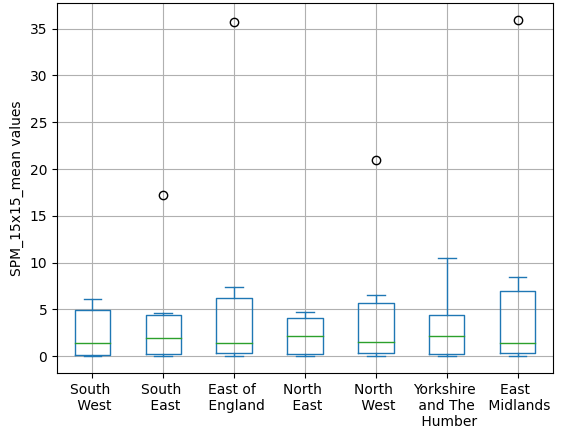
\includegraphics[height=0.5\textwidth]{images/spm_boxplot.png}
        \caption{Box plots depicting the distribution of mean SPM values at a 15x15 window for all S3 data, grouped by region. Green line indicates the median value, lower and upper bounds of the box refer to Q1 and Q3 values respectively, and the lowest and highest line refer to the minimum and maximum respectively, sans the outliers represented by circular dots.}
        \label{fig:spm_by_region}
\end{figure}


From the Table \ref{tab:metrics_across_years}, \ref{tab:metrics_across_months} and \ref{tab:metrics_across_regions}, it can be seen that 

\begin{enumerate}
    \item All models had the best performance for year 2020 and the worst performance for year 2022. Especially for Convolution Neural Network, which F1 Score dropped from 0.087 to 0.063
    \item All models had the best performance in September, and worst performance in May.
    \item All models had the best performance for North West region, and the worst performance for East of England.
\end{enumerate}

We believe that the main reason why all models had the same strengths and weaknesses across years, months and regions seems to be the proportion of positive labels for samples in each category. When there are more pollution incident reports, the classifiers make less mistakes. 

Figure \ref{fig:pc_by_year} and \ref{fig:pc_by_month} show the changes in the variables across years and months. The correlation trends in variables between different variables match the results of the previous EDA section, where we see that all values decrease over the years together except for ZSD. 

The distribution of SPM values in each region can be found in Figure \ref{fig:spm_by_region}. We chose SPM for this analysis due to its higher correlation with the sewage pollution risk in comparison to other variables, and because other variables (except ZSD) exhibit a very similar pattern. The region of North West England has the highest proportion of positive labels. SPM values within this region was also skewed towards relatively higher values and this region has the highest proportion of positive labels. It is interesting to note that for East of England and East Midlands, despite having a somewhat similar \% positive train and test as regions like South West and South East, has a significantly worser F1 score across all models. This suggests that perhaps the models perform worse on data points with higher SPM values overall, evident with how in \ref{fig:spm_by_region} East Midlands has a very high q3 and maximum value for average 15x15 SPM values. 

The conclusion we can make from Table \ref{tab:metrics_across_regions} and Figure \ref{fig:spm_by_region} is that the 'threshold' of SPM to discriminate between the pollution risk-level-normal or risk-level-increased varies across different regions. Within regions like East of England and East Midlands, the 'threshold' of SPM might be higher as the average level of SPM is generally higher. Conversely, for the regions like North West, the 'threshold' for SPM might be lower as the average values of SPM in this region are generally lower.

\subsection{Across Clusters in risk-level-increased data}
\label{sec:across_clusters}

In \hyperref[sec:clustering]{Section 2.3.3 (Clustering Analysis)}, K-means clustering suggested the risk-level-increased data could be categorized into two clusters. Here we would like to see how the models work for both clusters. Since only the samples where all features had at least one value within the 15x15 window were considered for the clustering analysis, lots of data were dropped. This meant that the test set only contained 100 samples that took part in the K-means clustering, which also meant the result was more likely to be noisy.

\begin{table}[h]
    \caption{Recall across test subsets from different clusters}
    \label{tab:metrics_across_clusters}
    \centering
    \begin{tabular}{lcccccc}
    \toprule
    \textbf{Cluster} & \textbf{Count positives} & \textbf{LR} & \textbf{RF} & \textbf{MLP} & \textbf{CNN} \\
    \midrule
    Cluster 1 & 43 & \textbf{2.33\%} & 2.33\% & \textbf{20.93\%} & \textbf{25.58\%} \\
    Cluster 2 & 57 & 0    & \textbf{5.26\%} & 0    & 7.02\% \\ \bottomrule
    \end{tabular}
\end{table}

In Table \ref{tab:metrics_across_clusters}, it can be seen that all models except Random Forest predicted better for Cluster 1. This difference was especially prominent for the neural network models, namely MLP and CNN. It appears that our models perform better on data points with large absolute values of all indicators (BBP, CDM, CHL, KD490, SPM) but ZSD, as is was observed for cluster 1 in figure \ref{fig:cluster_details}. In particular, the average value of SPM in cluster 1 was much higher than in risk-level-normal samples. 

In contrast, cluster 2 corresponds to the risk-level-increased instances with lower-than-average values of most indicators (BBP, CDM, CHL, KD490, SPM). A poorer performance on the data points in this cluster can correspond to the cases when an increased risk did not result in significant changes in the optical characteristics of the water and hence these cases are much harder to predict based on satellite imagery alone. 

\section{Gains From Feature Engineering}
\label{sec:Gains From Feature Engineering}

To better illustrate whether there are gains from feature engineering, we also ran a logistic regression and random forest model on our raw dataset, such that we could compare model performance from training and testing on raw S3 data versus engineered features S3 data for three broad categories of models: logistic regression, random forest and neural networks. The multi-layer perceptron model and convolutional neural network model represent a neural network model trained on engineered feature dataset and raw data respectively; thus for this comparison no additional neural network model was trained and results are instead compiled into the table from section 4.1 for ease of comparison.

To train logistic regression and random forest model on raw data, we created a dataset from the raw S3 dataset that turns each pixel within the 15 x 15 window for each variable into a feature, such that we have 6 x 15 x 15 = 1,350 features for each time-site pair. Although this is arguably still 'feature engineering', it does not involve aggregation as performed for our engineered feature dataset and preserves all data points in the raw data. Thus, it is referred to as 'raw' data here, and it should still provide an interesting comparison with the engineered feature dataset used.

Table \ref{tab:gains_from_feature_engineering} shows model performance for the three categories of models with raw data as outlined above and engineered features data. The two new models model was trained using either best parameter settings from section 4.1, or with default settings. 
    \begin{table}[h]
        \caption{Model Performance for 3 categories of models with raw data and engineered features data. Best best-performing classifier for each metric shown in bold.}
        \label{tab:gains_from_feature_engineering}
        \centering
        \begin{tabular}{lccccccc}
        \toprule
        \textbf{Model} & \textbf{Data} & \textbf{F1 Score} & \textbf{Precision} & \textbf{Recall} & \textbf{AP} & \textbf{ROC-AUC}  \\
        \midrule
        LR & Raw & 0.050 & \textbf{0.050} & 0.050 & 0.029 & 0.512  \\
         & EF & 0.073 & 0.039 & 0.610 & 0.034 & 0.597   \\ \midrule
        RF & Raw & 0.073 & 0.039 & 0.534 & \textbf{0.087} & \textbf{0.670}    \\
         & EF & \textbf{0.079} & 0.042 & 0.666 & 0.043 & 0.651  \\ \midrule
        NN & Raw & 0.077 & 0.041 & 0.668 & 0.040 & 0.627    \\
         & EF & 0.076 & 0.041 & \textbf{0.735} & 0.037 & 0.625    \\ \bottomrule
        \end{tabular}
    \end{table}

Comparing each category of models with different data, it appears the neural network on the raw data (CNN model from section 4.1) is marginally better compared to the neural network on the engineered features data (MLP model from section 4.1), yet we observe that the opposite seems to be the case for logistic regression and random forest models, with the difference being more significant for logistic regression than random forest. This seems to reflect that for neural networks, there are benefits to feeding the dataset more fine-grained data rather than simply aggregated data. By interpreting the data as an image, CNN can extract higher-level features from the data and generalise them across different time-site pairs. On the other hand, it seems like creating engineered features reduced noise in the data such that logistic regression and random forest were able to identify the positive class labels better. To classify with raw data for LR and RF, essentially these models compare the same pixel across windows identify the importance of that pixel in classification, and do this for each pixel individually. There are obvious flaws to this, as the orientation of the land and the ocean varies wildly across sites (see figure \ref{fig:selected15x15chl}), and thus the importance of different pixels varies across different sites. 

In addition, looking at our main evaluation metric of the f1 score, it is observed that the best overall model is still the random forest on engineered features data. This re-emphasizes how our dataset may have too few positive samples for neural networks to learn, as neural networks are known to be extremely data-hungry and also are difficult to train on unbalanced datasets, where random forest does not require as much data and can work on unbalanced datasets better.

For the other evaluation metrics, we observe that the best classifier differs from that of the f1 score. This reflects the tradeoff between many of the metrics for each model, with a key one being precision and recall. 

\section{Comparison between Sentinel 2 and Sentinel 3 Data}
\label{sec:Comparison between Sentinel 2 and Sentinel 3 Data}

We hoped to compare model performance differences in training and testing models on the S2 versus S3 dataset to gain insight into whether the higher resolution of the S2 dataset provides any additional gain and insight. 

To do so, for each of LR, RF, MLP and CNN we train and test a model on S2 data with a 51x51 window, while also rerunning the binary classifiers on modified S3 data with a 5x5 window. S3 data on a 5x5 window covers approximately \SI{5}km x \SI{5} km = \SI{25}{\km\squared}, which approximately overlaps that of the S2 51x51 windowed data, covering approximately \SI{5.1}km x \SI{5.1}km = \SI{26}{\km\squared}. Furthermore, we extracted a new set of time-site pairs for training and testing, where only time-site pairs that are present in both the S2 and S3 datasets (and in the bathing water dataset for risk-level labels) were used. The following table provides an overview of the new dataset.  


\begin{table}[h]
        \caption{Overview of Train and Test Datasets used for S2 \& S3 comparison}
        \label{table:s2s3_train_test}
        \centering
        \begin{tabular}{lcccc}
        \toprule
        \textbf{Dataset} & \textbf{Split \%} & \textbf{\# of Datapoints} &  \textbf{\# of Pos. Samples} & \textbf{\% of Pos. Samples} \\
        \midrule
        S2S3 Train & 80\% & 41,668 & 1,066 & 2.56\% \\
        S2S3 Test & 20\% & 10,557 & 302 & 2.86\% \\ 
        \midrule
        S2S3 & 100\% & 52,225 & 1,368 & 2.62\% \\
        \bottomrule
        \end{tabular}
\end{table}

To modify the S3 dataset, for LR, RF and MLP, all the features and metrics with window sizes larger than 5x5 were dropped from the dataset, and the models ran on the remaining data. For CNN, only data points in the centre 5x5 window were preserved, with the rest discarded. In order to use the same CNN architecture as the one used for our initial comparison in section 4.1, a padding of 0 was added around the 5x5 window for each of the 6 features such that the input tensor continues to have a dimension of 15x15x6. 

By comparing models from S2 and S3 data run on 1. the same area and 2. the same number of data points, we can better compare what are the effects of having more fine-grained data (S2) versus less fine-grained data (S3) on model performance. Table \ref{tab:s2_s3_model_comparison} displays the result of this analysis. 

    \begin{table}[h]
        \caption{Model Performance for LR, RF, MLP and CNN trained and tested on S2 versus S3 data, covering approximately the same area over the same time-site pairs.}
        \label{tab:s2_s3_model_comparison}
        \centering
        \begin{tabular}{lccccccc}
        \toprule
        \textbf{Model} & \textbf{Data} & \textbf{F1 Score} & \textbf{Precision} & \textbf{Recall} & \textbf{AP} & \textbf{ROC-AUC} \\
        \midrule
        LR & S2 51x51 & 0.105 & 0.059 & 0.467 & 0.043 & 0.624 \\
         & S3 5x5 & 0.090 & 0.050 & 0.542 & 0.040 & 0.622 \\ \midrule
        RF & S2 51x51 & \textbf{0.282} & \textbf{0.917}	& 0.167	& \textbf{0.353} & 0.790 \\
         & S3 5x5 & 0.021 & 0.026 & 0.018 & 0.029 & 0.500 \\ \midrule
        MLP & S2 51x51 & 0.128 & 0.072 & 0.606 & 0.055 & 0.687 \\
         & S3 5x5 & 0.091 & 0.049 & \textbf{0.702} & 0.043 & 0.654  \\ \midrule
        CNN & S2 51x51 & 0.085 & 0.064 & 0.254 & 0.057 & 0.629    \\
         & S3 5x5 & 0.089 & 0.052 & 0.623 & 0.050 & \textbf{0.689}   \\ \bottomrule
        \end{tabular}
    \end{table}

For all models except for CNN, we observe that the f1 score for the S2 model is significantly better than that of S3. This seems to show that having higher-resolution data is beneficial. This was especially the case for the random forest model, where we see an F1 score of 0.282, much higher than that observed in other classifiers previously. 

We note that CNN is an exception to the observation above, where the model performed slightly better on the lower-resolution S3 data. A reason for this could be due to how there are much more parameters in the CNN model for S2 data than for S3 data due to the substantial increase in window size. Typically models with more hyperparameters to learn require more data. With the same amount of time-site pairs, a model with more hyperparameters to learn may perform worse than one with less hyperparameters. This is less of an issue with the other models, as the number of hyperparameters to learn increases linearly with widow size, while for the neural network, it increased more than tenfold. 

Similarly, the best classifier for other metrics is somewhat different than that of the f1 score. It is perhaps interesting to note that precision is higher for the S2 data than for the S3 data for all classifiers. 

We thought it would also be interesting to directly compare S3 results on a 5x5 window as compared to a 15x15 window. This is presented in table \ref{tab:s3_5v15_model_comparison}. Note that this table does not contain any new data, but rather is a compilation of results from tables \ref{tab:all_hyperparameter_results} and \ref{tab:s2_s3_model_comparison}. 

    \begin{table}[h]
        \caption{Model Performance for LR, RF, MLP and CNN trained and tested on S3 5x5 and S3 15x15, covering the same time-site pairs.}
        \label{tab:s3_5v15_model_comparison}
        \centering
        \begin{tabular}{lccccccc}
        \toprule
        \textbf{Model} & \textbf{Data} & \textbf{F1 Score} & \textbf{Precision} & \textbf{Recall} & \textbf{AP} & \textbf{ROC-AUC} \\ \midrule
        LR & S3 5x5 & 0.090 & 0.050 & 0.542 & 0.040 & 0.622   \\ 
         & S3 15x15 & 0.073 & 0.039 & 0.610 & 0.034 & 0.597 \\ \midrule
        RF & S3 5x5 & 0.021 & 0.026 & 0.018 & 0.029 & 0.500 \\
         & S3 15x15 & 0.079 & 0.042 & 0.666 & 0.043 & 0.651  \\ \midrule
        MLP & S3 5x5 & \textbf{0.091} & 0.049 & 0.702 & 0.043 & 0.654   \\
         & S3 15x15 & 0.076 & 0.040 & \textbf{0.735} & 0.037 & 0.625  \\ \midrule
        CNN & S3 5x5 & 0.089 & \textbf{0.052} & 0.623 & \textbf{0.050} & \textbf{0.689}    \\ 
         & S3 15x15 & 0.077 & 0.041 & 0.668 & 0.040 & 0.627  \\ \bottomrule
        \end{tabular}
    \end{table}

It is interesting to see that for all models except for RF, we observe that S3 5x5 performs better than S3 15x15. We may argue that this shows that a lot more noise is introduced when we increase the window size to 15x15 from 5x5, which makes it difficult for the models to extract signals. 15x15 covers 15km x 15km, which is a rather large geographic area. It would appear that the RF is the best at extracting signals through the noise in this case. 

Furthermore, the best classifier, according to the F1 score, is the MLP on the 5x5 dataset. This signifies that there are still merits to running our data on more complex models that can model complex non-linear relationships. However, the reason CNN (which can also model complex non-linear relationships) perform worse than MLP could be due to insufficient data and thus a lower data-to-hyperparameter ratio than MLP. 

\section{Impact of Window Size}
\label{sec:Impact of Window Size}

Models were retrained using different window sizes to explore the relationship between window size and model performance. We hypothesised that we might see an increase in the f1 score with window size up to a certain 'optimal' window size, then decrease from there afterwards. It seems that getting more data surrounding the site would help explain sewage pollution up to a certain point until the window size becomes too large, and the additional noise from a larger window size makes it no longer possible to extract more signals. 

The training used the ‘cumulative’ window size features. For example, with a window size of 1x1, only the 1x1 features in the dataset were utilized. For a window size of 3x3, both 1x1 and 3x3 features were included in the training. Likewise, for a 5x5 window, features from 1x1, 3x3, and 5x5 were all used, and this approach continued for all window sizes from 1x1 to 15x15. This approach was adopted because, in the feature-engineered dataset, each feature represents statistics for data within that grid size, reflecting the general distribution of the data within that grid. Using only the data from the grid itself might result in a loss of useful information from the internal grid.

Features with cumulative window sizes ranging from 1x1 to 9x9 were extracted from the S2 dataset, and those from 1x1 to 15x15 were taken from the S3 dataset. These features were used to train all four models. The graph \ref{fig:window_size} depicts F1 scores of those four models and the baseline model denoted by legends, with the y-axis representing the scores and the x-axis showing the varying window sizes.

\begin{figure}[H]
\centering
\begin{subfigure}[b]{0.4\textwidth}
    \centering
    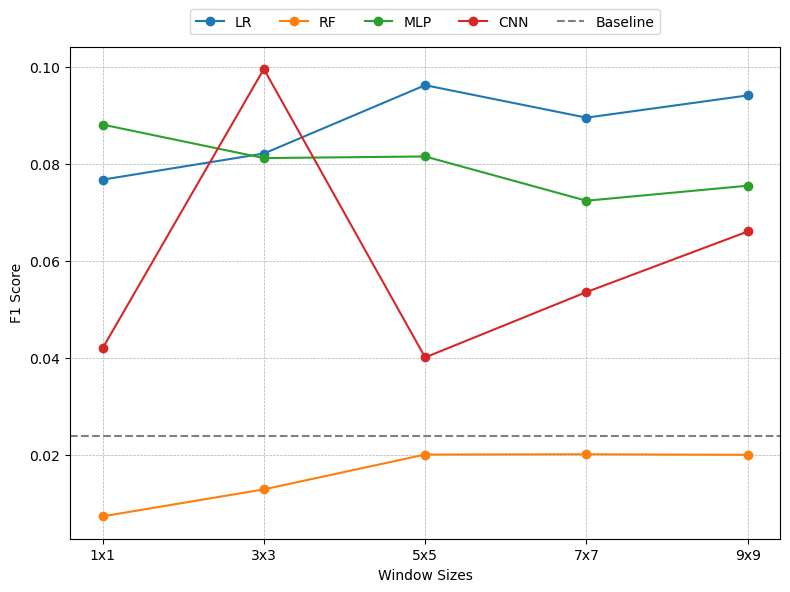
\includegraphics[width=\textwidth]{images/window_size_s2.png}
    \caption{Window size 1x1 to 9x9 comparison, S2}
    \label{fig:window_size_s2}
\end{subfigure}
  \hfill
\begin{subfigure}[b]{0.4\textwidth}
    \centering
    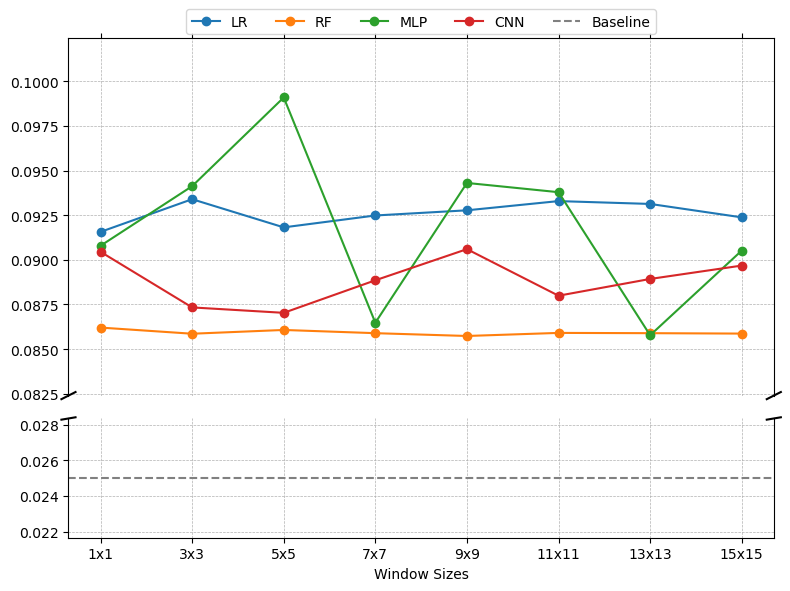
\includegraphics[width=\textwidth]{images/window_size_s3.png}
    \caption{Window size 1x1 to 15x15 comparison, S3}
    \label{fig:window_size_s3}
\end{subfigure}
\caption{Model Performance Comparison by Window Size}
\label{fig:window_size}
\end{figure}


All models demonstrated a fluctuating pattern as the window size expanded. No consistent trend of performance was observed, suggesting a complex relationship between window size and model performance. 

In the context of the S2 dataset, the F1 scores for LR, RF, and MLP remained relatively stable across different window sizes. The CNN model's F1 score, however, exhibited pronounced variability. It peaked at the '3x3', significantly decreased at '5x5', and then gradually rebounded by '9x9'. Random Forest showed the poorest performance compared to other models when comparing across window sizes. This seems contrary to our previous findings, where the Random Forest yielded the best performance. This discrepancy might be due to the fact that the dataset used here only included records available for both S2 and S3 data. We then took a subset using window sizes, which could have resulted in a significant reduction in data size. Random Forest is sensitive to such changes, leading to this differing result.

 On the other hand, within the S3 dataset, LR, RF, and CNN consistently maintained their F1 scores across window sizes. While MLP displayed considerable fluctuations in its performance across window sizes, oscillating with high variability and no apparent pattern. 


Our initial assumption that model performance would increase and then decrease as window sizes increase was not observed. There are two potential reasons for why we may not have seen this initial increase. Firstly, perhaps the optimal window size is somewhere in between 1km x 1km and 3km x 3km, or potentially even smaller than 1km x 1km. S3 data does not give us enough granularity to check if this is the case. Secondly, it may be that increasing the window size increases model complexity for the models by increasing number of parameters to be learnt or increasing size of the model, such that without increasing the number of time-site pairs model performance overall declines despite additional signal from an increased window size. This argument appears more likely to be true for neural network than for other models. Reasons for not seeing a strong subsequent decrease include perhaps not expanding the window size enough to see additional noise overwhelm signal, or perhaps that the models are actually relatively good at ignoring noise from a larger window size. 

Overall, while we observe some fluctuations in model performance from altering window size, the fluctuations are either insignificant or lack a clear trend. 

\chapter{Conclusion and Extensions}

Making sewage pollution predictions from satellite data can significantly increase efficiency and reduce cost of monitoring sewage pollution. This project aims to investigate how we can best build models to extract sewage pollution signals from satellite data by comparing and evaluating several binary classifiers that take satellite data as input and outputs whether there is sewage pollution or not. 

To conclude, we found that the performance of the best binary classifiers exceeds the baseline model, and we were able to draw several interesting findings from comparing and evaluating numerous classifiers with different settings. We report that our best-performing classifier in terms of f1 score is the random forest model on the engineered features dataset from Sentinel-2 data with a 51x51 window, with an f1 score of 0.282. 

Our main findings are summarised as follows: 

Among the models examined, Random Forest stands out, demonstrating the best capability in predicting water pollution risk. Its performance remains consistent regardless of using -10 or 0 as placeholders for missing values, designating it as the optimal choice for the S3 data. Meanwhile, for the other binary classifiers, replacing missing values with -10 in the S3 dataset shows better effectiveness in enhancing predictive capabilities than using 0. This observation could serve as a benchmark for subsequent experimentation of other models.

Model performance varies based on the category being examined, whether it's by year, month, or region. Within the scope of our research and dataset, model performance tends to decrease year by year but increases monthly during the bathwater season (from May to September). The east coast of England displayed poorer performance compared to other regions across all models. Data imbalance appears to influence these performances significantly. Moreover, of the two clusters in the 'risk-level-increased' data, models generally predicted better for cluster 1 (which has higher average values than most 'risk-level-normal' data for all features except ZSD, while cluster 2 is the opposite), with the exception of the Random Forest model.

Feature engineering plays a significant role in enhancing the performance of certain models. Specifically, while neural networks, particularly CNNs, seem to benefit from raw, detailed data, traditional algorithms like logistic regression and random forest exhibit improved performances with engineered features, where noise is reduced and essential patterns are captured. For the given dataset, the random forest model trained on engineered features provided the most promising results, highlighting its robustness even in situations with limited data and imbalances.

Higher-resolution data, as in Sentinel 2 (S2), typically results in improved model performance, notably regarding F1 scores and precision. However, even with its higher resolution, CNN demonstrated marginally better results on Sentinel 3 (S3) data. This implies that an increase in model parameters, without a corresponding rise in data, may diminish performance. Similarly, while more complex models like MLP can potentially excel in identifying complex data patterns, sufficient data remains critical for optimal performance.

While the initial hypothesis that model performance would follow a curve of increasing and then decreasing with larger window sizes was not supported by the findings. Increased window sizes made models more complex without necessarily improving performance, and Multi-layer Perceptron and Neural Networks might be more affected by this complexity than other models. In essence, while some performance fluctuations were observed with changes in window size, they were not significant or did not follow a predictable trend.

Ultimately, it is perhaps unfortunate that even the best classifiers observed had somewhat subpar performance, where many of the classifiers have very high False Positive Rate, despite many attempts to refine and improve the models. We believe that we faced several limitations, including computational and time constraints, which made it more difficult to obtain better results. In the following section, we suggest several improvements that we believe would improve and make our results more robust, as well as suggest ideas for further research. 

\section{Improvements and Further Research}
This section outlines several improvements and extensions that can be made to achieve better results.

\noindent \textbf{Run models on more historical data.} 
Getting more historical data to increase the dataset size temporally is a natural extension of our investigations and is likely to lead to an improvement in classifier performance. The impact is likely to be especially prominent for the neural network models, which are known to be more data-hungry. 

\noindent \textbf{Incorporating lagged historic data.}
Lagged satellite data could be added, such that sewage pollution predictions are made not only from today's satellite data but also from satellite data from yesterday. This would transform the model into one involving time series and would require additional analyses and care. 

\noindent \textbf{Incorporate More Signals.}
Potential confounding variables that are expected to influence satellite observations but are unrelated to sewage pollution can be added to help the model cut through the noise in the data. For example, adding wind, precipitation or other weather-related data could help control for changes in observed CHL values etc. due to weather conditions. Bathymetry data can also be incorporated to control for ocean depth. 

\noindent \textbf{Created more sophisticated binary classifiers.}
Model complexity and architecture could be further improved especially for the neural network models (MLP and CNN), which in conjunction with using more data could lead to improvements in the model. 

\noindent \textbf{Improve model tuning.}
The time-consuming nature of iteratively tuning the binary classifiers with grid search means that we may have been unable to get to the optimal classifiers for most model types. Perhaps some improvements in results can be achieved with a more systematic and efficient method of tuning hyperparameters, such as expanding the search space with random search. Cross-validation could also be implemented with more time and computational resources.

\noindent \textbf{Regression instead of Classification.}
This project focused on binary classifiers for ease of interpretation, but the bathing water data provided by the environment agency also contains lab-tested water sample results that indicate whether there is pollution or not. A regression model could be built instead with the continuous, numerical water sample results. It would be interesting to see if a regression model might perform better than a binary classifier on this dataset.

\noindent \textbf{Ensemble Models.}
Given how we noticed classifier performance differing across categories in section \ref{sec:Strengths and Weaknesses of Best Models}, exploring ensemble models could be an interesting extension. Perhaps classifier performance can be improved by training classifiers on subsets of the dataset, and then combining multiple classifiers together for a final predictive model. For example, if a datapoint belongs in May-July, classifier 1 would be used, whereas if the datapoint belongs in August-September, classifier 2 would be used. 

\noindent \textbf{Incorporating Sewage Pollution Data from Other Countries.} The project can be extended to make predictions on sewage pollution for the coastlines of other countries. Copernicus data covers an extensive area across the globe; although different countries have different ways of measuring sewage pollution and it may be difficult to align these measures. 



\bibliographystyle{agsm}

\bibliography{references}

\begin{comment}
\appendix
\chapter{Detailed Model Performance Across Years, Months and Regions}
\section{CNN}
\begin{table}[h]
        \caption{Model Performance Across Years}
        \label{tab:cnn_across_years}
        \centering
        \begin{tabular}{lccccccc}
        \toprule
        \textbf{Year} & \textbf{Count} & \textbf{F1 Score} & \textbf{ROC-AUC} & \textbf{PR-AUC} & \textbf{Precision} & \textbf{Recall} & \textbf{Accuracy} \\
        \midrule
        2020 & 11766 & 0.087 & 0.046 & 0.702 & 0.042 & 0.621 & 0.545 \\
        2021 & 12894 & 0.079 & 0.042 & 0.639 & 0.038 & 0.587 & 0.538  \\ 
        2022 & 12763 & 0.063 & 0.033 & 0.663 & 0.029 & 0.623 & 0.586 \\ \bottomrule
        \end{tabular}
    \end{table}

     \begin{table}[h]
        \caption{Model Performance Across Months}
        \label{tab:cnn_across_months}
        \centering
        \begin{tabular}{lccccccc}
        \toprule
        \textbf{Year} & \textbf{Count} & \textbf{F1 Score} & \textbf{ROC-AUC} & \textbf{PR-AUC} & \textbf{Precision} & \textbf{Recall} & \textbf{Accuracy} \\
        \midrule
        May & 6430 & 0.053 & 0.027 & 0.717 & 0.024 & 0.66 & 0.604 \\
        June & 7690 & 0.059 & 0.031 & 0.704 & 0.028 & 0.619 & 0.537  \\ 
        July & 7829 & 0.055 & 0.028 & 0.671 & 0.026 & 0.604 & 0.54 \\
        August & 7683 & 0.095 & 0.051 & 0.664 & 0.045 & 0.615 & 0.569 \\
        September & 7429 & 0.113 & 0.062 & 0.645 & 0.056 & 0.592 & 0.544 \\ \bottomrule
        \end{tabular}
    \end{table}

    \begin{table}[h]
        \caption{Model Performance Across Regions}
        \label{tab:cnn_across_regions}
        \centering
        \begin{tabular}{lccccccc}
        \toprule
        \textbf{Year} & \textbf{Count} & \textbf{F1 Score} & \textbf{ROC-AUC} & \textbf{PR-AUC} & \textbf{Precision} & \textbf{Recall} & \textbf{Accuracy} \\
        \midrule
        South West & 17926 & 0.071 & 0.037 & 0.65 & 0.033 & 0.613 & 0.578 \\
        South East & 7603 & 0.08 & 0.042 & 0.665 & 0.037 & 0.632 & 0.602  \\ 
        East of England & 3510 & 0.044 & 0.023 & 0.569 & 0.021 & 0.558 & 0.547 \\
        North East & 2953 & 0.101 & 0.054 & 0.815 & 0.049 & 0.676 & 0.546 \\
        North West & 2557 & 0.12 & 0.065 & 0.748 & 0.062 & 0.585 & 0.438 \\
        Yorkshire & 1832 & 0.074 & 0.04 & 0.5 & 0.039 & 0.512 & 0.523 \\
        East Midlands & 696 & 0.047 & 0.025 & 0.55 & 0.026 & 0.453 & 0.362 \\ 
        London & 346 & 0.078 & 0.04 & 1.0 & 0.04 & 0.5 & 0.04 \\ \bottomrule
        \end{tabular}
    \end{table}

\section{RF}
\begin{table}[h]
        \caption{Model Performance Across Years}
        \label{tab:cnn_across_years}
        \centering
        \begin{tabular}{lccccccc}
        \toprule
        \textbf{Year} & \textbf{Count} & \textbf{F1 Score} & \textbf{ROC-AUC} & \textbf{PR-AUC} & \textbf{Precision} & \textbf{Recall} & \textbf{Accuracy} \\
        \midrule
        2020 & 11766 & 0.086 & 0.647 & 0.049 & 0.046 & 0.677 & 0.565 \\
        2021 & 12894 & 0.084 & 0.637 & 0.049 & 0.045 & 0.668 & 0.560  \\ 
        2022 & 12763 & 0.064 & 0.668 & 0.033 & 0.034 & 0.648 & 0.612 \\ \bottomrule
        \end{tabular}
    \end{table}

     \begin{table}[h]
        \caption{Model Performance Across Months}
        \label{tab:cnn_across_months}
        \centering
        \begin{tabular}{lccccccc}
        \toprule
        \textbf{Year} & \textbf{Count} & \textbf{F1 Score} & \textbf{ROC-AUC} & \textbf{PR-AUC} & \textbf{Precision} & \textbf{Recall} & \textbf{Accuracy} \\
        \midrule
        May & 6430 & 0.053 & 0.690 & 0.035 & 0.027 & 0.708 & 0.619 \\
        June & 7690 & 0.058 & 0.643 & 0.030 & 0.031 & 0.682 & 0.560  \\ 
        July & 7829 & 0.062 & 0.670 & 0.036 & 0.032 & 0.732 & 0.580 \\
        August & 7683 & 0.095 & 0.647 & 0.060 & 0.051 & 0.636 & 0.593 \\
        September & 7429 & 0.114 & 0.630 & 0.062 & 0.063 & 0.647 & 0.556 \\ \bottomrule
        \end{tabular}
    \end{table}

    \begin{table}[h]
        \caption{Model Performance Across Regions}
        \label{tab:cnn_across_regions}
        \centering
        \begin{tabular}{lccccccc}
        \toprule
        \textbf{Year} & \textbf{Count} & \textbf{F1 Score} & \textbf{ROC-AUC} & \textbf{PR-AUC} & \textbf{Precision} & \textbf{Recall} & \textbf{Accuracy} \\
        \midrule
        South West & 17926 & 0.074 & 0.674 & 0.043 & 0.039 & 0.637 & 0.626 \\
        South East & 7603 & 0.082 & 0.668 & 0.044 & 0.044 & 0.684 & 0.606  \\ 
        East of England & 3510 & 0.043 & 0.583 & 0.023 & 0.022 & 0.656 & 0.463 \\
        North East & 2953 & 0.102 & 0.698 & 0.106 & 0.055 & 0.739 & 0.595 \\
        North West & 2557 & 0.120 & 0.585 & 0.089 & 0.077 & 0.702 & 0.471 \\
        Yorkshire & 1832 & 0.082 & 0.546 & 0.077 & 0.056 & 0.543 & 0.535 \\
        East Midlands & 696 & 0.063 & 0.578 & 0.052 & 0.045 & 0.737 & 0.402 \\ 
        London & 346 & 0.078 & 0.500 & 0.520 & 0.040 & 1.000 & 0.040 \\ \bottomrule
        \end{tabular}
    \end{table}

\end{comment}
\end{document}